% =====================================================================
%  Anatomía de un LLM — Fase IV — Módulo 16
%  Preentrenamiento a escala
%  Compilar: latexmk -r ../latexmkrc M16-escala.tex
% =====================================================================
\documentclass[11pt,a4paper,twoside,openany]{book}
\usepackage{../estilo-apuntes}

\newcommand{\ApuntesCurso}{Anatomía de un LLM}
\newcommand{\ApuntesModulo}{Módulo 16}

\hypersetup{pdftitle={Módulo 16. Preentrenamiento a escala},pdfauthor={Anatomía de un LLM}}

% Notación propia del módulo
\newcommand{\T}{^{\top}}
\newcommand{\Var}{\operatorname{Var}}
\newcommand{\PP}{\mathbb{P}}
\newcommand{\Nopt}{N_{\mathrm{opt}}}
\newcommand{\Dopt}{D_{\mathrm{opt}}}
\newcommand{\Loss}{\mathcal{L}}
\newcommand{\sig}{\operatorname{sig}}
\newcommand{\nctx}{n_{\mathrm{ctx}}}

\begin{document}
\frontmatter
% ------------------------------------------------------------------ Portada
\begin{titlepage}
\centering
\vspace*{2.5cm}
{\large\scshape Anatomía de un LLM}\par
\vspace{0.4cm}
{\normalsize Fundamentos matemáticos de los modelos de lenguaje}\par
\vspace{2.2cm}
\rule{\textwidth}{0.8pt}\par\vspace{0.5cm}
{\small\scshape Fase IV \textperiodcentered\ Escala, sistemas y arquitecturas modernas}\par\vspace{0.3cm}
{\Huge\bfseries Módulo 16\par}\vspace{0.3cm}
{\LARGE Preentrenamiento a escala\par}
\vspace{0.5cm}\rule{\textwidth}{0.4pt}\par
\vspace{1.6cm}
{\large Apuntes del curso}\par
\vfill
{\small Edición de octubre de 2026}\par
\end{titlepage}

% ------------------------------------------------------- Presentación
\chapter*{Presentación del módulo}
\addcontentsline{toc}{chapter}{Presentación del módulo}
\markboth{Presentación del módulo}{}

Los módulos~14 y~15 construyeron un Transformer, contaron su coste y lo entrenaron a pequeña escala. Este módulo estudia qué ocurre cuando el mismo procedimiento se lleva a billones de tokens y a decenas de miles de millones de parámetros. La pregunta central es económica: con un presupuesto de cómputo $C$ fijo, ¿qué tamaño de modelo $N$ y qué número de tokens $D$ conviene elegir, y de dónde salen esos tokens? La respuesta tiene dos partes. La primera es la ingeniería de los datos: filtrar la web, eliminar duplicados con MinHash y LSH y mezclar fuentes. La segunda son las \emph{leyes de escalado}, relaciones empíricas en forma de ley de potencia entre la pérdida y los recursos, que permiten plantear el reparto como un problema de optimización con restricciones y resolverlo con multiplicadores de Lagrange. El módulo termina con dos cuestiones abiertas: si las capacidades «emergentes» son reales y qué cuesta ampliar la ventana de contexto.

\section*{Objetivos}
Al finalizar el módulo, el estudiante debe ser capaz de:
\begin{enumerate}[label=\arabic*.]
  \item describir las etapas de preparación de un corpus de preentrenamiento, aplicar reglas heurísticas de calidad, relacionar el filtro por perplejidad con la entropía cruzada y calcular las épocas de cada fuente de una mezcla;
  \item definir la similitud de Jaccard, demostrar la propiedad fundamental de MinHash, obtener la varianza de su estimador y analizar la curva en S del LSH por bandas;
  \item caracterizar las leyes de potencia, ajustarlas por mínimos cuadrados en escala log-log y enunciar las leyes de escalado de Kaplan \emph{et al.};
  \item derivar con multiplicadores de Lagrange el reparto óptimo de Chinchilla entre $N$ y $D$, demostrar sus consecuencias y justificar la regla de unos 20 tokens por parámetro;
  \item explicar los tres métodos empíricos de Hoffmann \emph{et al.}, incorporar el coste de inferencia y la repetición de datos al reparto y calcular cuándo se amortiza sobreentrenar un modelo pequeño;
  \item analizar el argumento de la métrica sobre las capacidades emergentes y cuantificar el coste en cómputo, memoria y codificación posicional del contexto largo.
\end{enumerate}

\section*{Requisitos previos}
Del módulo~1, la entropía cruzada, la perplejidad y la desigualdad de Gibbs (tema~5). Del módulo~4, los multiplicadores de Lagrange y la convexidad. Del módulo~5, la independencia, la distribución binomial y la varianza de una media. Del módulo~6, la divergencia de Kullback--Leibler. Del módulo~7, los calendarios de tasa de aprendizaje con decaimiento coseno. Del módulo~8, la regresión lineal por mínimos cuadrados. Del módulo~12, la tokenización. Del módulo~13, el coste cuadrático de la atención. Del módulo~14, la regla $C\approx 6ND$, el coste $2N$ por token de la inferencia y RoPE (temas~4 y~6). Del módulo~15, el bucle de entrenamiento y las curvas de pérdida.

\section*{Organización}
\begin{center}
\small
\begin{tabular}{@{}cll@{}}
\toprule
Tema & Contenido & Fuentes principales \\
\midrule
1 & Datos de preentrenamiento & \cite{rae}, \cite{wenzek}, \cite{fineweb}, \cite{llama}, \cite{cs336a4} \\
2 & Deduplicación: MinHash y LSH & \cite{mmds}, \cite{cs246}, \cite{broder}, \cite{lee}, \cite{cs336a4} \\
3 & Leyes de potencia y leyes de Kaplan & \cite{kaplan}, \cite{cs324}, \cite{cs336a3} \\
4 & El reparto óptimo del cómputo: Chinchilla & \cite{hoffmann}, \cite{bv}, \cite{cs336a3} \\
5 & Estimación empírica, inferencia y datos limitados & \cite{hoffmann}, \cite{muennighoff}, \cite{sardana}, \cite{cs336a3} \\
6 & Capacidades emergentes y contexto largo & \cite{wei}, \cite{schaeffer}, \cite{chenpi}, \cite{llama3} \\
\bottomrule
\end{tabular}
\end{center}

Cada tema termina con una lista de lecturas y con ejercicios graduados en tres niveles: $\star$ comprensión, $\star\star$ cálculo y $\star\star\star$ demostración. Los ejercicios marcados con \emph{Fuente} están adaptados de cursos y libros de texto universitarios; el enunciado se ha redactado de nuevo y, en algunos casos, se han cambiado los datos para que puedan resolverse a mano. Las soluciones completas, paso a paso, están en el \cref{ap:soluciones}.

\section*{Sobre las fuentes}
El texto es de redacción propia. La deduplicación sigue el capítulo~3, «Finding Similar Items», de Leskovec, Rajaraman y Ullman~\cite{mmds}, libro de texto del curso CS246 de Stanford~\cite{cs246}, y la sección~3 de la práctica de datos del curso CS336 de Stanford~\cite{cs336a4}. Las leyes de escalado siguen los artículos originales de Kaplan \emph{et al.}~\cite{kaplan} y de Hoffmann \emph{et al.}~\cite{hoffmann}, la clase sobre leyes de escalado del curso CS324 de Stanford~\cite{cs324} y la práctica de leyes de escalado de CS336~\cite{cs336a3}; la forma convexa del problema de reparto procede de la programación geométrica de Boyd y Vandenberghe~\cite[§4.5]{bv}. Los datos sobre corpus reales proceden de los informes de Gopher~\cite{rae}, LLaMA~\cite{llama,llama2,llama3}, RefinedWeb~\cite{refinedweb} y FineWeb~\cite{fineweb}; la repetición de datos, de Muennighoff \emph{et al.}~\cite{muennighoff}; las capacidades emergentes, de Wei \emph{et al.}~\cite{wei} y Schaeffer, Miranda y Koyejo~\cite{schaeffer}. Anthropic, Google y xAI no publican el tamaño ni la composición de los corpus de Claude, Gemini y Grok; sobre ellos solo se usa información pública~\cite{gemini15}.

\section*{Notación}
\begin{center}
\begin{tabular}{@{}ll@{}}
\toprule
Símbolo & Significado \\
\midrule
$N$, $D$, $C$ & parámetros, tokens de entrenamiento y FLOPs de entrenamiento \\
$L$, $L(N,D)$ & pérdida de validación (nats por token) y su ley de escalado \\
$E$, $A$, $B$, $\alpha$, $\beta$ & constantes de la ley de Chinchilla \\
$\Nopt(C)$, $\Dopt(C)$ & reparto óptimo para el presupuesto $C$ \\
$w_i$, $U_i$, $e_i$ & peso, tokens únicos y épocas de la fuente $i$ de una mezcla \\
$J(A,B)$ & similitud de Jaccard de dos conjuntos \\
$h$, $\sig(S)$ & función hash y firma MinHash del conjunto $S$ \\
$b$, $r$ & bandas y filas por banda del LSH ($n=br$ funciones hash) \\
$k$ & longitud de una respuesta en tokens o de un \emph{shingle} \\
$n$, $\nctx$ & longitud de la secuencia y ventana de contexto \\
$\ln$, $\log_{10}$ & logaritmo natural y decimal \\
\bottomrule
\end{tabular}
\end{center}

Las pérdidas se miden en nats por token. Se usa la escala numérica larga del español: un \emph{billón} es $10^{12}$ y mil millones, $10^{9}$.

\tableofcontents

\mainmatter
% =====================================================================
\chapter{Datos de preentrenamiento}
\label{tema:1}
% =====================================================================

El preentrenamiento minimiza la entropía cruzada media sobre un corpus (módulo~1, tema~5), de modo que el modelo aprende la distribución del texto que se le muestra. La composición de ese corpus es, por tanto, una decisión de diseño tan importante como la arquitectura. Este tema describe cómo se obtiene un corpus a partir de la web y formaliza tres de sus etapas: los filtros de calidad, el filtro por perplejidad y la mezcla de fuentes. Se siguen las secciones~2 y~4 de la práctica de datos de CS336~\cite{cs336a4}, la clase sobre datos de CS324~\cite{cs324} y los informes de CCNet~\cite{wenzek}, Gopher~\cite[§3.4 y apéndice~A]{rae}, RefinedWeb~\cite[§3]{refinedweb}, FineWeb~\cite{fineweb} y LLaMA~\cite[§2.1]{llama}. La deduplicación, que también forma parte del proceso, se estudia por separado en el \cref{tema:2}.

\section{Del rastreo web al corpus}

\begin{definicion}[Corpus de preentrenamiento]
Un \emph{corpus de preentrenamiento} es una colección finita de documentos $\mathcal{C}=\{x^{(1)},\dots,x^{(M)}\}$, cada uno una secuencia de tokens. Su \emph{tamaño} es el número total de tokens, $\sum_{m}\abs{x^{(m)}}$. Un \emph{filtro} es un predicado $f$ sobre documentos; aplicarlo a $\mathcal{C}$ produce $\{x\in\mathcal{C}:f(x)=1\}$. Un proceso de preparación es una composición de transformaciones (extracción, normalización) y filtros.
\end{definicion}

La fuente principal es la web. Common Crawl publica volcados periódicos de miles de millones de páginas; FineWeb, por ejemplo, se construyó a partir de 96 volcados y contiene unos $15$ billones de tokens~\cite{fineweb}. La \cref{fig:proceso} resume las etapas habituales. Casi todo el material en bruto se descarta: en RefinedWeb, la identificación del idioma elimina cerca de la mitad de los documentos, y el conjunto del proceso, casi el $90\,\%$~\cite[§3 y figura~2]{refinedweb}.

\begin{figure}[h]
\centering
\begin{tikzpicture}[font=\small,
  caja/.style={draw,rounded corners=2pt,align=center,minimum height=9mm,text width=2.25cm,inner sep=2pt},
  flecha/.style={-{Stealth[length=2mm]},thick}]
  \node[caja] (a) {Rastreo\\(HTML)};
  \node[caja,right=0.45cm of a] (b) {Extracción\\del texto};
  \node[caja,right=0.45cm of b] (c) {Identificación\\del idioma};
  \node[caja,right=0.45cm of c] (d) {Filtros de\\calidad};
  \node[caja,below=0.9cm of d] (e) {Deduplicación\\(\cref{tema:2})};
  \node[caja,left=0.45cm of e] (f) {Datos personales\\y toxicidad};
  \node[caja,left=0.45cm of f] (g) {Mezcla de\\fuentes};
  \node[caja,left=0.45cm of g] (h) {Tokenización\\(módulo~12)};
  \draw[flecha] (a)--(b); \draw[flecha] (b)--(c); \draw[flecha] (c)--(d);
  \draw[flecha] (d)--(e); \draw[flecha] (e)--(f); \draw[flecha] (f)--(g); \draw[flecha] (g)--(h);
\end{tikzpicture}
\caption{Etapas habituales de la preparación de un corpus a partir de la web, según~\cite{cs336a4,refinedweb,fineweb}. El orden concreto varía de un informe a otro.}
\label{fig:proceso}
\end{figure}

\section{Filtros heurísticos de calidad}

Los filtros más sencillos son reglas sobre estadísticas superficiales del documento. Son baratos, deterministas y fáciles de auditar. El informe de Gopher~\cite[apéndice~A]{rae} define un conjunto de ellas; la práctica de CS336~\cite[§2.6]{cs336a4} usa el siguiente subconjunto.

\begin{definicion}[Filtros de Gopher, subconjunto de CS336]\label{def:gopher}
Un documento con $W$ palabras, longitud media de palabra $\bar{\ell}$ (en caracteres) y $\Lambda$ líneas \emph{pasa} el filtro si se cumplen las cuatro condiciones siguientes:
\begin{enumerate}
  \item $50\le W\le 100\,000$;
  \item $3\le\bar{\ell}\le 10$;
  \item como mucho el $30\,\%$ de las $\Lambda$ líneas termina en puntos suspensivos;
  \item al menos el $80\,\%$ de las palabras contiene un carácter alfabético.
\end{enumerate}
\end{definicion}

\begin{ejemplo}\label{ej:gopher}
Un documento de $120$ palabras y $480$ caracteres en palabras, con $10$ líneas, $4$ de las cuales terminan en «...», tiene $\bar{\ell}=480/120=4$, pero una fracción de líneas truncadas de $4/10=0{,}40>0{,}30$. No pasa el filtro: es típico de las páginas de listados con fragmentos de artículos.
\end{ejemplo}

\section{Filtro por perplejidad}

CCNet~\cite{wenzek} puntúa cada página con un modelo de $n$-gramas entrenado sobre Wikipedia y conserva las de perplejidad baja; LLaMA usó este proceso para su parte de Common Crawl~\cite[§2.1]{llama}. La idea es que el texto parecido al de referencia recibe probabilidad alta. El caso de un modelo de unigramas permite analizar exactamente qué mide el filtro.

\begin{definicion}[Perplejidad de un documento]
Sea $q$ una distribución sobre $\V$ con $q(v)>0$ para todo $v$ (un modelo de unigramas de referencia) y sea $x=(x_1,\dots,x_T)$ un documento. La perplejidad de $x$ según $q$ es
\[
\PPL_q(x)=\exp\Bigl(-\frac1T\sum_{t=1}^{T}\ln q(x_t)\Bigr).
\]
La \emph{distribución empírica} de $x$ es $\hat p_x(v)=\abs{\{t:x_t=v\}}/T$.
\end{definicion}

\begin{proposicion}\label{prop:ppl-kl}
Para todo documento $x$,
\[
\ln\PPL_q(x)=H(\hat p_x,q)=H(\hat p_x)+D(\hat p_x\,\|\,q).
\]
\end{proposicion}

\begin{proof}
Agrupando las posiciones por token, $\sum_{t}\ln q(x_t)=\sum_{v}T\hat p_x(v)\ln q(v)$. Dividiendo por $-T$ se obtiene $-\sum_v\hat p_x(v)\ln q(v)=H(\hat p_x,q)$, la entropía cruzada (módulo~1, tema~5). La segunda igualdad es la descomposición $H(p,q)=H(p)+D(p\,\|\,q)$ del módulo~6, que se comprueba sumando y restando $\sum_v\hat p_x(v)\ln\hat p_x(v)$.
\end{proof}

La \cref{prop:ppl-kl} muestra que el filtro premia dos cosas distintas: que el documento se parezca a la referencia (divergencia pequeña) y que el documento sea poco variado (entropía empírica pequeña). La segunda es indeseable.

\begin{corolario}[El filtro premia la repetición]\label{cor:repeticion}
Sea $q_{\max}=\max_v q(v)$. Para todo documento $x$, $\PPL_q(x)\ge 1/q_{\max}$, con igualdad si y solo si todos los tokens de $x$ maximizan $q$.
\end{corolario}

\begin{proof}
Cada factor cumple $-\ln q(x_t)\ge-\ln q_{\max}$, luego la media también, y $\PPL_q(x)\ge e^{-\ln q_{\max}}=1/q_{\max}$. La igualdad en la media exige la igualdad en cada término, es decir, $q(x_t)=q_{\max}$ para todo $t$.
\end{proof}

\begin{ejemplo}\label{ej:ppl-filtro}
Sea $q(\texttt{a})=0{,}5$, $q(\texttt{b})=0{,}3$, $q(\texttt{c})=0{,}2$. El documento «a b a c» tiene $\PPL_q=(0{,}5\cdot 0{,}3\cdot 0{,}5\cdot 0{,}2)^{-1/4}=0{,}015^{-1/4}=2{,}857$. Su distribución empírica es $(1/2,1/4,1/4)$, con $H(\hat p)=1{,}0397$ nats y $D(\hat p\,\|\,q)=0{,}0102$ nats; la suma, $1{,}0499$, es $\ln 2{,}857$, como predice la \cref{prop:ppl-kl}. El documento degenerado «a a a a» obtiene la perplejidad mínima, $1/0{,}5=2$. Por eso los procesos reales combinan el filtro por perplejidad con reglas contra la repetición~\cite[apéndice~A]{rae}.
\end{ejemplo}

\section{Clasificadores de calidad}

Una alternativa es aprender qué es «calidad» a partir de ejemplos. Se toman como positivos documentos de una fuente de referencia (por ejemplo, páginas citadas desde Wikipedia) y como negativos páginas aleatorias de Common Crawl, y se entrena un clasificador lineal~\cite[§2.7]{cs336a4}.

\begin{definicion}[Filtro por clasificador]
Sea $g\colon\mathcal{X}\to[0,1]$ un clasificador que estima la probabilidad de que un documento proceda de la fuente de referencia. El filtro con umbral $\tau$ conserva los documentos con $g(x)\ge\tau$. Subir $\tau$ aumenta la precisión y reduce la cobertura.
\end{definicion}

LLaMA entrenó un clasificador lineal que distingue las páginas usadas como referencia en Wikipedia de páginas aleatorias, y descartó las no clasificadas como referencia~\cite[§2.1]{llama}. FineWeb-Edu sustituye la fuente de referencia por anotaciones de un modelo grande: Llama-3-70B-Instruct puntuó el «valor educativo» de una muestra de páginas de $0$ a $5$, se ajustó una regresión sobre embeddings y se conservaron las páginas con puntuación al menos~$3$, unos $1{,}3$ billones de tokens~\cite[§4]{fineweb}.

\begin{observacion}
«Calidad» es una elección, no una propiedad objetiva del texto. Un clasificador entrenado con Wikipedia como modelo de lo deseable tiende a descartar registros informales, variedades dialectales e idiomas con pocos recursos, y el modelo resultante hereda ese sesgo. Las reglas heurísticas tienen el mismo problema en menor grado: un umbral de longitud media de palabra pensado para el inglés no es neutral para otros idiomas.
\end{observacion}

\section{Mezcla de fuentes y épocas}

El corpus final combina varias fuentes (web, código, libros, artículos científicos, Wikipedia) con pesos fijados por experimentos.

\begin{definicion}[Mezcla y épocas]\label{def:mezcla}
Sean $m$ fuentes con $U_i$ tokens únicos cada una y sean $w_i\ge 0$, $\sum_i w_i=1$, los \emph{pesos de muestreo}. Un entrenamiento de $D$ tokens extrae $w_iD$ tokens de la fuente $i$; su número de \emph{épocas} es
\[
e_i=\frac{w_iD}{U_i}.
\]
Si $e_i>1$, la fuente se \emph{sobremuestrea}: parte de su texto se ve varias veces.
\end{definicion}

\begin{proposicion}\label{prop:factible}
Sea $E_{\max}>0$. Existe una mezcla con $e_i\le E_{\max}$ para todo $i$ si y solo si $D\le E_{\max}\sum_{i}U_i$.
\end{proposicion}

\begin{proof}
Si $e_i\le E_{\max}$ para todo $i$, entonces $w_iD\le E_{\max}U_i$; sumando sobre $i$ y usando $\sum_iw_i=1$, $D\le E_{\max}\sum_iU_i$. Recíprocamente, si se cumple la desigualdad, los pesos proporcionales $w_i=U_i/\sum_jU_j$ dan $e_i=D/\sum_jU_j\le E_{\max}$ para todo $i$.
\end{proof}

\begin{ejemplo}[La mezcla de LLaMA]\label{ej:llama-mezcla}
La tabla~1 de~\cite{llama} da, para el entrenamiento de $1{,}4$ billones de tokens, el peso y las épocas de cada fuente. Despejando $U_i=w_iD/e_i$ se obtienen los tokens únicos implícitos:
\begin{center}\small
\begin{tabular}{@{}lrrrr@{}}
\toprule
Fuente & $w_i$ & $e_i$ & $w_iD$ ($10^{9}$) & $U_i=w_iD/e_i$ ($10^{9}$) \\
\midrule
CommonCrawl & $0{,}670$ & $1{,}10$ & $938$ & $853$ \\
C4 & $0{,}150$ & $1{,}06$ & $210$ & $198$ \\
GitHub & $0{,}045$ & $0{,}64$ & $63$ & $98$ \\
Wikipedia & $0{,}045$ & $2{,}45$ & $63$ & $26$ \\
Libros & $0{,}045$ & $2{,}23$ & $63$ & $28$ \\
ArXiv & $0{,}025$ & $1{,}06$ & $35$ & $33$ \\
StackExchange & $0{,}020$ & $1{,}03$ & $28$ & $27$ \\
\bottomrule
\end{tabular}
\end{center}
Wikipedia y los libros, fuentes pequeñas y valiosas, se recorren más de dos veces; parte de GitHub no llega a verse. El \cref{tema:5} cuantifica cuánto vale un token repetido: hasta unas cuatro épocas, casi lo mismo que uno nuevo~\cite{muennighoff}.
\end{ejemplo}

\section{La escala de los datos}

La \cref{tab:tokens-param} recoge la relación entre tokens de entrenamiento y parámetros de varios modelos con informe público. El cambio entre 2020 y 2023 se explica en los temas~\ref{tema:4} y~\ref{tema:5}.

\begin{table}[h]
\centering\small
\caption{Parámetros, tokens de entrenamiento y tokens por parámetro.}\label{tab:tokens-param}
\begin{tabular}{@{}lrrr@{}}
\toprule
Modelo (referencia) & $N$ & $D$ & $D/N$ \\
\midrule
GPT-3~\cite{brown} & $1{,}75\cdot 10^{11}$ & $3\cdot 10^{11}$ & $1{,}7$ \\
Gopher~\cite{rae} & $2{,}8\cdot 10^{11}$ & $3\cdot 10^{11}$ & $1{,}1$ \\
Chinchilla~\cite{hoffmann} & $7\cdot 10^{10}$ & $1{,}4\cdot 10^{12}$ & $20$ \\
LLaMA 7B~\cite{llama} & $6{,}7\cdot 10^{9}$ & $10^{12}$ & $149$ \\
Llama~2 7B~\cite{llama2} & $6{,}74\cdot 10^{9}$ & $2\cdot 10^{12}$ & $297$ \\
Llama~3 405B~\cite{llama3} & $4{,}05\cdot 10^{11}$ & $1{,}56\cdot 10^{13}$ & $38{,}5$ \\
\bottomrule
\end{tabular}
\end{table}

\begin{lecturas}
\item Stanford CS336~\cite{cs336a4}, práctica~4 «Data», §2.6 «Quality Rules», §2.7 «Quality Classifier» y §4 «Filter data for language modeling».
\item Stanford CS324~\cite{cs324}, clase «Data».
\item Wenzek \emph{et al.}~\cite{wenzek}, CCNet: filtro por perplejidad con modelos de $n$-gramas.
\item Penedo \emph{et al.}~\cite{refinedweb}, §3, y~\cite{fineweb}, §3 y §4: procesos completos sobre Common Crawl.
\item Touvron \emph{et al.}~\cite{llama}, §2.1 «Pre-training Data», tabla~1.
\end{lecturas}

\section*{Ejercicios del tema 1}
\addcontentsline{toc}{section}{Ejercicios del tema 1}

\begin{ejercicio}{1}{eje:1-sesgo}
Un equipo entrena un clasificador de calidad con páginas citadas desde la Wikipedia en inglés como ejemplos positivos y lo aplica a un rastreo multilingüe. Indique dos tipos de texto que el filtro tenderá a descartar injustificadamente y una consecuencia para el modelo resultante. ¿Qué medida reduciría el problema?
\end{ejercicio}

\begin{ejercicio}{1}{eje:1-gopher}
Aplique los filtros de la \cref{def:gopher} a los cuatro documentos siguientes y decida cuáles pasan.
\begin{center}\small
\begin{tabular}{@{}lrrrrr@{}}
\toprule
Doc. & Palabras & Caracteres en palabras & Líneas & Líneas con «...» & Palabras con letra \\
\midrule
A & $40$ & $200$ & $4$ & $0$ & $38$ \\
B & $1200$ & $5640$ & $60$ & $24$ & $1170$ \\
C & $800$ & $4160$ & $50$ & $6$ & $720$ \\
D & $3000$ & $13\,500$ & $100$ & $5$ & $2250$ \\
\bottomrule
\end{tabular}
\end{center}
\fuente{adaptado de Stanford CS336~\cite{cs336a4}, práctica~4, §2.6, problema \texttt{gopher\_quality\_filters} (se sustituye la implementación por el cálculo).}
\end{ejercicio}

\begin{ejercicio}{2}{eje:1-mezcla}
Se entrena con $D=10^{12}$ tokens una mezcla de cuatro fuentes: web ($8\cdot 10^{11}$ tokens únicos, peso $0{,}60$), código ($2\cdot 10^{11}$, $0{,}25$), libros ($5\cdot 10^{10}$, $0{,}10$) y ciencia ($10^{10}$, $0{,}05$). Calcule las épocas de cada fuente. ¿Cuál preocupa, si se acepta un máximo de unas $4$ épocas? Proponga un ajuste de pesos.
\end{ejercicio}

\begin{ejercicio}{2}{eje:1-ppl}
Un modelo de unigramas de referencia asigna $q(\text{de})=0{,}4$, $q(\text{la})=0{,}3$, $q(\text{casa})=0{,}2$ y $q(\text{oferta})=0{,}1$. Calcule la perplejidad de los documentos A~=~«la casa de la», B~=~«oferta oferta oferta casa» y C~=~«de de de de». ¿Cuáles conserva un filtro con umbral $\PPL\le 4$? Compruebe la \cref{prop:ppl-kl} para el documento~A.
\end{ejercicio}

\begin{ejercicio}{2}{eje:1-fermi}
Un proceso de filtrado procesa $2500$ archivos WET de Common Crawl en $1{,}5$ horas en una máquina. Supóngase que un volcado completo tiene $100\,000$ archivos WET. (a) ¿Cuánto tarda en filtrarse un volcado en esa máquina? (b) ¿Cuántas máquinas hacen falta para filtrarlo en $2$ horas? (c) ¿Cuántas horas-máquina requieren los $96$ volcados de FineWeb?
\fuente{adaptado de Stanford CS336~\cite{cs336a4}, práctica~4, §4, problema \texttt{filter\_data}, apartado~(b) (con tiempos supuestos).}
\end{ejercicio}

\begin{ejercicio}{3}{eje:1-minmax}
Con la notación de la \cref{def:mezcla}, demuestre que, para $D$ fijo, la mezcla que minimiza el máximo de las épocas, $\max_ie_i$, es la proporcional, $w_i=U_i/\sum_jU_j$, y que es la única. Calcule ese mínimo para la mezcla de LLaMA del \cref{ej:llama-mezcla} y compárelo con las épocas de Wikipedia elegidas por sus autores.
\end{ejercicio}

% =====================================================================
\chapter{Deduplicación: MinHash y LSH}
\label{tema:2}
% =====================================================================

La web contiene muchas copias del mismo texto: páginas idénticas, plantillas, licencias que solo cambian en el año y el autor, artículos reproducidos con otro pie de página. Este tema estudia cómo detectarlas a escala de miles de millones de documentos. Los duplicados exactos se resuelven con funciones hash; los casi duplicados, con la similitud de Jaccard, las firmas MinHash y el \emph{hashing} sensible a la localidad (LSH). Se sigue el capítulo~3 de Leskovec, Rajaraman y Ullman~\cite{mmds} (§3.1, §3.3 y §3.4), las clases «Locality-Sensitive Hashing~I y~II» del curso CS246~\cite{cs246} y la sección~3 de la práctica de datos de CS336~\cite{cs336a4}. MinHash procede de Broder~\cite{broder}.

\section{Por qué deduplicar}

Lee \emph{et al.}~\cite{lee} mostraron que eliminar duplicados de corpus estándar reduce la frecuencia con que el modelo reproduce texto literal del entrenamiento y permite alcanzar la misma calidad con menos pasos. Hay tres razones complementarias.

\begin{enumerate}
  \item \emph{Cómputo.} Con un presupuesto $C\approx 6ND$ fijo (módulo~14), cada token repetido ocupa el lugar de uno nuevo.
  \item \emph{Memorización.} Lo que aparece cientos de veces se aprende literalmente y puede regurgitarse, incluidos datos personales o protegidos.
  \item \emph{Contaminación.} Si un documento de evaluación tiene copias en el corpus de entrenamiento, las métricas se inflan.
\end{enumerate}

\section{Duplicados exactos}

\begin{definicion}[Huella]
Sea $H\colon\Sigma^{*}\to\{0,1\}^{\ell}$ una función hash de $\ell$ bits (por ejemplo, SHA-1 o MD5). La \emph{huella} de un documento normalizado $x$ es $H(x)$. La deduplicación exacta conserva un documento por huella, con un recorrido y un diccionario de huellas: coste lineal en el tamaño del corpus.
\end{definicion}

\begin{proposicion}[Colisiones]\label{prop:colisiones}
Supóngase que $H$ asigna a cada uno de $M$ documentos distintos un valor uniforme e independiente en $\{0,1\}^{\ell}$. El número esperado de pares de documentos distintos con la misma huella es $\binom{M}{2}2^{-\ell}$.
\end{proposicion}

\begin{proof}
Para cada par $\{i,j\}$ sea $I_{ij}$ la indicatriz de $H(x^{(i)})=H(x^{(j)})$. Fijado el valor de $H(x^{(i)})$, la probabilidad de que $H(x^{(j)})$ coincida es $2^{-\ell}$, luego $\E[I_{ij}]=2^{-\ell}$. Por la linealidad de la esperanza, el número esperado de colisiones es $\sum_{i<j}\E[I_{ij}]=\binom{M}{2}2^{-\ell}$.
\end{proof}

Con $M=10^{9}$ documentos hay $\binom{M}{2}\approx 5\cdot 10^{17}$ pares: una huella de $64$ bits produce en promedio $0{,}027$ colisiones, y una de $128$ bits, $1{,}5\cdot 10^{-21}$. La deduplicación exacta también puede hacerse por líneas: se cuentan las apariciones de cada línea en el corpus y se eliminan las repetidas, lo que borra cabeceras, menús y pies de página~\cite[§3.1]{cs336a4}. Llama~3 elimina las líneas que aparecen más de seis veces en cada grupo de $30$ millones de documentos~\cite[§3.1.1]{llama3}.

\section{Shingles y similitud de Jaccard}

Dos páginas que solo difieren en la fecha tienen huellas distintas. Para detectar casi duplicados se representa cada documento por un conjunto y se mide el solapamiento~\cite[§3.1]{mmds}.

\begin{definicion}[Shingles]
Sea $k\ge 1$. El conjunto de \emph{$k$-shingles} de un documento de palabras $(u_1,\dots,u_T)$ es $S_k=\{(u_t,\dots,u_{t+k-1}):1\le t\le T-k+1\}$, el conjunto de grupos de $k$ palabras consecutivas.
\end{definicion}

\begin{definicion}[Similitud de Jaccard]
Sean $A$ y $B$ conjuntos finitos, no ambos vacíos. Su \emph{similitud de Jaccard} es
\[
J(A,B)=\frac{\abs{A\cap B}}{\abs{A\cup B}}\in[0,1].
\]
Vale~$1$ si y solo si $A=B$ y vale~$0$ si y solo si son disjuntos. La \emph{distancia de Jaccard} $1-J(A,B)$ es una distancia en el sentido métrico~\cite[cap.~3]{mmds}.
\end{definicion}

\begin{ejemplo}\label{ej:jaccard}
Con $2$-shingles, «el gato duerme en el sofá» da $\{$el gato, gato duerme, duerme en, en el, el sofá$\}$ y «el gato duerme en la cama» da $\{$el gato, gato duerme, duerme en, en la, la cama$\}$. Comparten $3$ shingles y la unión tiene $5+5-3=7$, de modo que $J=3/7\approx 0{,}429$.
\end{ejemplo}

Comparar todos los pares de $M=10^{9}$ documentos exige unos $5\cdot 10^{17}$ cálculos de $J$, inabordable. Las dos secciones siguientes resuelven, respectivamente, el coste de almacenar los conjuntos y el de compararlos todos.

\section{Firmas MinHash}

\begin{definicion}[MinHash]
Sea $\Omega$ un universo finito que contiene todos los shingles y sea $\pi$ una permutación de $\Omega$, identificada con una biyección $\pi\colon\Omega\to\{1,\dots,\abs{\Omega}\}$. El \emph{minhash} de un conjunto no vacío $S\subseteq\Omega$ es $h_\pi(S)=\min_{x\in S}\pi(x)$. Con $n$ permutaciones $\pi_1,\dots,\pi_n$, la \emph{firma} de $S$ es el vector $\sig(S)=\bigl(h_{\pi_1}(S),\dots,h_{\pi_n}(S)\bigr)$.
\end{definicion}

\begin{teorema}[Propiedad fundamental de MinHash]\label{teo:minhash}
Si $\pi$ es una permutación uniforme de $\Omega$ y $A,B\subseteq\Omega$ son no vacíos,
\[
\PP\bigl(h_\pi(A)=h_\pi(B)\bigr)=J(A,B).
\]
\end{teorema}

\begin{proof}
Sea $x^{*}$ el elemento de $A\cup B$ con menor valor de $\pi$. Como $\pi$ es uniforme, cada elemento de $A\cup B$ tiene la misma probabilidad, $1/\abs{A\cup B}$, de ser el primero de $A\cup B$ en el orden de $\pi$, luego $x^{*}$ es uniforme en $A\cup B$. Si $x^{*}\in A\cap B$, es el mínimo tanto de $A$ como de $B$ y los minhash coinciden. Si $x^{*}\in A\setminus B$, entonces $h_\pi(A)=\pi(x^{*})$, mientras que $h_\pi(B)=\pi(y)$ para algún $y\in B$ distinto de $x^{*}$, y $\pi(y)\neq\pi(x^{*})$ porque $\pi$ es inyectiva; los minhash difieren. El caso $x^{*}\in B\setminus A$ es simétrico. Por tanto, los minhash coinciden si y solo si $x^{*}\in A\cap B$, suceso de probabilidad $\abs{A\cap B}/\abs{A\cup B}$.
\end{proof}

\begin{corolario}[Estimador de Jaccard]\label{cor:estimador}
Sean $\pi_1,\dots,\pi_n$ permutaciones uniformes e independientes y sea $\hat J$ la fracción de coordenadas en que coinciden $\sig(A)$ y $\sig(B)$. Entonces $n\hat J\sim\mathrm{Bin}(n,J)$, con $J=J(A,B)$; en particular,
\[
\E[\hat J]=J\qquad\text{y}\qquad\Var(\hat J)=\frac{J(1-J)}{n}.
\]
\end{corolario}

\begin{proof}
Cada coordenada coincide con probabilidad $J$ por el \cref{teo:minhash}, de forma independiente porque las permutaciones lo son. El número de coincidencias es una suma de $n$ variables de Bernoulli independientes de parámetro $J$, es decir, una binomial (módulo~5). Dividiendo por $n$, $\E[\hat J]=nJ/n=J$ y $\Var(\hat J)=nJ(1-J)/n^{2}=J(1-J)/n$.
\end{proof}

Con $n=100$ funciones, la desviación típica es como mucho $\sqrt{0{,}25/100}=0{,}05$. La firma sustituye un conjunto de miles de shingles por $n$ enteros. En la práctica, las permutaciones se aproximan con funciones hash de una misma familia con semillas distintas~\cite[§3.2]{cs336a4}: calcular $\min_{x\in S}h(x)$ requiere un único recorrido de $S$.

\section{LSH por bandas}

\begin{definicion}[LSH por bandas]
Sea $n=br$. Se divide la firma en $b$ bandas de $r$ coordenadas consecutivas. Dos documentos son \emph{candidatos} si sus firmas coinciden en todas las coordenadas de al menos una banda. En la práctica se asigna cada banda de cada documento a un cubo mediante una función hash, y solo se comparan los documentos que comparten algún cubo.
\end{definicion}

\begin{proposicion}[Curva en S]\label{prop:curva-s}
Sean dos documentos con similitud de Jaccard $s$ y firmas construidas con permutaciones independientes. La probabilidad de que sean candidatos es
\[
P(s)=1-\bigl(1-s^{r}\bigr)^{b}.
\]
La función $P$ es creciente en $[0,1]$, con $P(0)=0$ y $P(1)=1$; vale $1/2$ en $s_{1/2}=(1-2^{-1/b})^{1/r}$ y, si $r\ge 2$ y $b\ge 2$, tiene un único punto de inflexión en $(0,1)$,
\[
s^{*}=\Bigl(\frac{r-1}{rb-1}\Bigr)^{1/r}.
\]
\end{proposicion}

\begin{proof}
Por el \cref{teo:minhash} y la independencia, las $r$ coordenadas de una banda coinciden con probabilidad $s^{r}$, y la banda falla con probabilidad $1-s^{r}$. Las $b$ bandas usan permutaciones distintas, luego fallan todas con probabilidad $(1-s^{r})^{b}$, y $P(s)$ es el complementario. La derivada $P'(s)=br\,s^{r-1}(1-s^{r})^{b-1}$ es positiva en $(0,1)$. Despejando $P(s)=1/2$ se obtiene $(1-s^{r})^{b}=1/2$, es decir, $s^{r}=1-2^{-1/b}$. Para la inflexión, se anula la derivada de $\ln P'(s)=\ln(br)+(r-1)\ln s+(b-1)\ln(1-s^{r})$:
\[
\frac{r-1}{s}-\frac{(b-1)rs^{r-1}}{1-s^{r}}=0\iff(r-1)(1-s^{r})=(b-1)rs^{r}\iff s^{r}=\frac{r-1}{rb-1}.
\]
La función $(r-1)/s-(b-1)rs^{r-1}/(1-s^{r})$ es estrictamente decreciente en $(0,1)$, pasa de $+\infty$ a $-\infty$ y cambia de signo una sola vez, de modo que $P'$ crece hasta $s^{*}$ y decrece después.
\end{proof}

Cuando $r$ es grande, $(r-1)/(rb-1)\to 1/b$, y se recupera la aproximación habitual del umbral, $s^{*}\approx(1/b)^{1/r}$~\cite[§3.4]{mmds}. Los pares con $s$ muy por debajo del umbral casi nunca se comparan y los pares con $s$ muy por encima casi siempre (\cref{fig:curva-s}).

\begin{figure}[h]
\centering
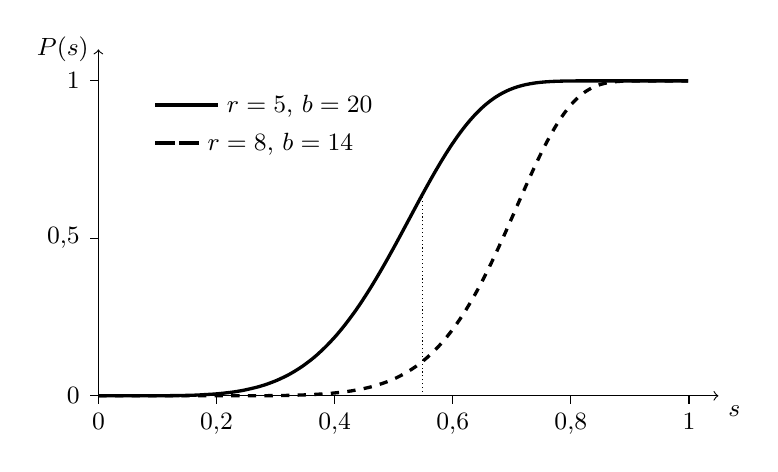
\begin{tikzpicture}[x=7.5cm,y=4cm,font=\small]
  \draw[->] (0,0)--(1.05,0) node[below right] {$s$};
  \draw[->] (0,0)--(0,1.1) node[left] {$P(s)$};
  \foreach \t in {0,0.2,0.4,0.6,0.8,1} \draw (\t,0)--(\t,-0.025) node[below] {\pgfmathprintnumber[use comma]{\t}};
  \foreach \t in {0,0.5,1} \draw (0,\t)--(-0.015,\t) node[left] {\pgfmathprintnumber[use comma]{\t}};
  \draw[very thick,domain=0:1,samples=120,smooth] plot (\x,{1-(1-\x^5)^20});
  \draw[very thick,dashed,domain=0:1,samples=120,smooth] plot (\x,{1-(1-\x^8)^14});
  \draw[densely dotted] (0.549,0)--(0.549,0.64);
  \node[anchor=west] at (0.08,0.92) {\rule[2pt]{8mm}{1.2pt}\ $r=5$, $b=20$};
  \node[anchor=west] at (0.08,0.80) {\rule[2pt]{2.5mm}{1.2pt}\,\rule[2pt]{2.5mm}{1.2pt}\ $r=8$, $b=14$};
\end{tikzpicture}
\caption{Curva en S de la \cref{prop:curva-s} para $(r,b)=(5,20)$ (continua; la línea punteada marca $(1/b)^{1/r}\approx 0{,}549$) y para la configuración de FineWeb, $(r,b)=(8,14)$ (discontinua).}
\label{fig:curva-s}
\end{figure}

\begin{ejemplo}[FineWeb]\label{ej:fineweb}
FineWeb calcula $112$ minhash sobre los $5$-gramas de palabras de cada documento y los agrupa en $b=14$ bandas de $r=8$~\cite[§3.4]{fineweb}. Para un par con $s=0{,}75$, $s^{8}=0{,}1001$ y $P=1-0{,}8999^{14}=0{,}772$, el valor del orden del $77\,\%$ que declara el artículo. La inflexión está en $s^{*}=(7/111)^{1/8}=0{,}708$. Los autores observaron además que deduplicar cada volcado por separado funcionaba mejor que deduplicar los $96$ volcados conjuntamente, que eliminaba hasta el $90\,\%$ de los datos antiguos.
\end{ejemplo}

\begin{lecturas}
\item Leskovec, Rajaraman y Ullman~\cite{mmds}, cap.~3 «Finding Similar Items», §3.1 a §3.4.
\item Stanford CS246~\cite{cs246}, clases «Locality-Sensitive Hashing~I» y «Locality-Sensitive Hashing~II».
\item Stanford CS336~\cite{cs336a4}, práctica~4, §3 «Deduplication» (problemas \texttt{exact\_deduplication} y \texttt{minhash\_deduplication}).
\item Broder~\cite{broder}, artículo original de MinHash.
\item Lee \emph{et al.}~\cite{lee}, efecto de la deduplicación sobre la memorización.
\end{lecturas}

\section*{Ejercicios del tema 2}
\addcontentsline{toc}{section}{Ejercicios del tema 2}

\begin{ejercicio}{1}{eje:2-porque}
¿Por qué un corpus con muchos duplicados es peor que uno deduplicado del mismo tamaño en tokens? Dé dos razones y un caso límite que las ilustre.
\end{ejercicio}

\begin{ejercicio}{1}{eje:2-conjuntos}
Calcule la similitud de Jaccard de cada par de conjuntos entre $S_1=\{a,b,c,d\}$, $S_2=\{b,c,e\}$ y $S_3=\{a,c,e,f\}$. ¿Qué par es el más parecido?
\fuente{adaptado de Leskovec, Rajaraman y Ullman~\cite{mmds}, cap.~3, ejercicio~3.1.1 (conjuntos modificados).}
\end{ejercicio}

\begin{ejercicio}{2}{eje:2-luna}
Calcule la similitud de Jaccard con $2$-shingles entre «la luna brilla sobre el mar» y «la luna brilla sobre el río». Explique por qué el resultado debe ser menor que $4/5$.
\end{ejercicio}

\begin{ejercicio}{2}{eje:2-firmas}
El universo es $\{0,1,2,3,4,5\}$, con $S_1=\{0,2,5\}$, $S_2=\{1,2,3\}$ y $S_3=\{0,3,5\}$. Se usan $h_1(x)=(x+1)\bmod 6$, $h_2(x)=(5x+1)\bmod 6$ y $h_3(x)=(2x+3)\bmod 6$. (a) ¿Cuáles de ellas son permutaciones del universo? (b) Calcule la firma MinHash de cada conjunto. (c) Compare la similitud estimada con la real para cada par.
\fuente{adaptado de Leskovec, Rajaraman y Ullman~\cite{mmds}, cap.~3, ejercicio~3.3.3 (conjuntos y funciones modificados).}
\end{ejercicio}

\begin{ejercicio}{2}{eje:2-lsh}
En un LSH con $r=4$ filas y $b=25$ bandas, calcule la probabilidad de que dos documentos sean candidatos si $s=0{,}3$ y si $s=0{,}85$. Calcule el umbral aproximado $(1/b)^{1/r}$ y el punto de inflexión exacto de la \cref{prop:curva-s}.
\end{ejercicio}

\begin{ejercicio}{2}{eje:2-curvas}
Para $(r,b)=(3,10)$, $(6,20)$ y $(5,50)$: (a) calcule $P(s)$ en $s=0{,}2$, $0{,}5$ y $0{,}8$; (b) calcule el valor exacto $s_{1/2}$ en que $P=1/2$ y compárelo con la aproximación $(1/b)^{1/r}$.
\fuente{adaptado de Leskovec, Rajaraman y Ullman~\cite{mmds}, cap.~3, ejercicios~3.4.1 y~3.4.2.}
\end{ejercicio}

\begin{ejercicio}{3}{eje:2-varianza}
(a) Demuestre que, para todo $J\in[0,1]$, la desviación típica del estimador del \cref{cor:estimador} es a lo sumo $1/(2\sqrt n)$. (b) Halle el menor $n$ que garantiza una desviación típica no mayor que $0{,}05$ para cualquier par de documentos, y el menor que la garantiza para pares con $J=0{,}8$. (c) Use la desigualdad de Chebyshev para acotar $\PP(\abs{\hat J-J}\ge 0{,}1)$ con $n=100$.
\end{ejercicio}

% =====================================================================
\chapter{Leyes de potencia y leyes de escalado de Kaplan}
\label{tema:3}
% =====================================================================

Kaplan \emph{et al.}~\cite{kaplan} observaron en 2020 que la pérdida de validación de un Transformer disminuye como una ley de potencia en cada uno de tres recursos, el número de parámetros $N$, el número de tokens $D$ y el cómputo $C$, a lo largo de varios órdenes de magnitud. Este tema estudia primero las leyes de potencia como objeto matemático (por qué son las funciones invariantes por cambio de escala y cómo se ajustan) y después enuncia las leyes de Kaplan y su recomendación de reparto. Se sigue~\cite[§1.2, §4 y §6]{kaplan}, la clase «Scaling laws» del curso CS324~\cite{cs324} y la revisión de leyes de escalado de la práctica~3 de CS336~\cite[§2]{cs336a3}.

\section{Leyes de potencia}

\begin{definicion}[Ley de potencia]
Una función $f\colon(0,\infty)\to(0,\infty)$ es una \emph{ley de potencia} si existen $c>0$ y $\alpha\in\R$ tales que $f(x)=c\,x^{-\alpha}$ para todo $x>0$. El número $\alpha$ es el \emph{exponente}; si $\alpha>0$, $f$ es decreciente.
\end{definicion}

La propiedad que distingue a las leyes de potencia es que no tienen escala característica: multiplicar $x$ por un factor $\lambda$ multiplica $f$ por un factor que no depende del punto de partida.

\begin{proposicion}[Invariancia de escala]\label{prop:escala}
Sea $f\colon(0,\infty)\to(0,\infty)$ continua. Existe una función $g$ con $f(\lambda x)=g(\lambda)f(x)$ para todos $\lambda,x>0$ si y solo si $f$ es una ley de potencia. En ese caso, $g(\lambda)=\lambda^{-\alpha}$.
\end{proposicion}

\begin{proof}
Si $f(x)=cx^{-\alpha}$, entonces $f(\lambda x)=c\lambda^{-\alpha}x^{-\alpha}=\lambda^{-\alpha}f(x)$. Recíprocamente, con $x=1$ se obtiene $g(\lambda)=f(\lambda)/f(1)$, de modo que $F=f/f(1)$ cumple $F(\lambda x)=F(\lambda)F(x)$. Sea $\varphi(t)=\ln F(e^{t})$, continua en $\R$. Entonces $\varphi(s+t)=\ln F(e^{s}e^{t})=\varphi(s)+\varphi(t)$: es la ecuación funcional de Cauchy. Por inducción, $\varphi(mt)=m\varphi(t)$ para $m\in\mathbb{N}$; de ahí $\varphi(p/q)=(p/q)\varphi(1)$ para todo racional positivo, y $\varphi(0)=0$, $\varphi(-t)=-\varphi(t)$ extienden la igualdad a todos los racionales. Por continuidad y densidad de $\mathbb{Q}$, $\varphi(t)=-\alpha t$ con $\alpha=-\varphi(1)$. Deshaciendo el cambio, $F(x)=x^{-\alpha}$ y $f(x)=f(1)\,x^{-\alpha}$.
\end{proof}

\begin{corolario}\label{cor:factor}
Si $L=cN^{-\alpha}$, cada vez que $N$ se multiplica por $\lambda$ la pérdida se multiplica por $\lambda^{-\alpha}$, sea cual sea $N$. En particular, la mejora relativa por cada duplicación de $N$ es constante, $1-2^{-\alpha}$.
\end{corolario}

\section{Ajuste en escala log-log}

\begin{proposicion}\label{prop:loglog}
$L=cN^{-\alpha}$ si y solo si $\log L=\log c-\alpha\log N$. En el plano $(u,v)=(\log N,\log L)$, una ley de potencia es una recta de pendiente $-\alpha$, en cualquier base del logaritmo.
\end{proposicion}

\begin{proof}
Se aplica el logaritmo, que es inyectivo, y se usan $\log(xy)=\log x+\log y$ y $\log x^{a}=a\log x$. El cambio de base multiplica $u$ y $v$ por la misma constante, que no altera la pendiente.
\end{proof}

En consecuencia, el exponente se estima por regresión lineal de $v$ sobre $u$ (módulo~8).

\begin{definicion}[Ajuste de una ley de potencia]\label{def:ajuste}
Dados entrenamientos $(N_j,L_j)$, $j=1,\dots,m$, con $u_j=\log N_j$ y $v_j=\log L_j$, el ajuste por mínimos cuadrados en escala log-log es la recta $v=b_0+b_1u$ con
\[
b_1=\frac{\sum_j(u_j-\bar u)(v_j-\bar v)}{\sum_j(u_j-\bar u)^{2}},\qquad b_0=\bar v-b_1\bar u,
\]
y la ley ajustada es $\hat L(N)=10^{b_0}N^{b_1}$ (con $\log=\log_{10}$), de exponente $\hat\alpha=-b_1$.
\end{definicion}

\begin{observacion}
El ajuste en escala logarítmica minimiza errores \emph{relativos}, no absolutos, y da el mismo peso a cada orden de magnitud. Es lo adecuado cuando los entrenamientos están espaciados geométricamente, como es habitual. Extrapolar es otra cuestión: una recta ajustada en $10^{7}$--$10^{9}$ parámetros y usada en $10^{11}$ supone que nada cambia en dos órdenes de magnitud sin observar.
\end{observacion}

\section{Las leyes de Kaplan}

Kaplan \emph{et al.}\ entrenaron Transformers decoder-only sobre WebText2 y midieron la entropía cruzada de validación en nats por token sobre contextos de $1024$ tokens~\cite[§2]{kaplan}. El número de parámetros $N$ excluye los embeddings de vocabulario y de posición~\cite[§1.3]{kaplan}.

\begin{definicion}[Leyes de Kaplan]\label{def:kaplan}
Cuando el crecimiento de la pérdida está limitado por un único recurso, la pérdida sigue~\cite[ecuaciones~(1.1)--(1.3)]{kaplan}
\[
L(N)=\Bigl(\frac{N_c}{N}\Bigr)^{\alpha_N},\qquad
L(D)=\Bigl(\frac{D_c}{D}\Bigr)^{\alpha_D},\qquad
L(C_{\min})=\Bigl(\frac{C_c}{C_{\min}}\Bigr)^{\alpha_C},
\]
con los valores ajustados de la \cref{tab:kaplan}. La ley en $N$ supone datos suficientes y entrenamiento hasta la convergencia; la ley en $D$, un modelo grande con parada temprana; la ley en $C_{\min}$, el mejor reparto posible del cómputo.
\end{definicion}

\begin{table}[h]
\centering\small
\caption{Constantes de las leyes de Kaplan \emph{et al.}~\cite[§1.2]{kaplan}. Un PF-día son $10^{15}\cdot 86\,400=8{,}64\cdot 10^{19}$ FLOP.}\label{tab:kaplan}
\begin{tabular}{@{}lll@{}}
\toprule
Ley & Exponente & Constante \\
\midrule
$L(N)$ & $\alpha_N\approx 0{,}076$ & $N_c\approx 8{,}8\cdot 10^{13}$ parámetros \\
$L(D)$ & $\alpha_D\approx 0{,}095$ & $D_c\approx 5{,}4\cdot 10^{13}$ tokens \\
$L(C_{\min})$ & $\alpha_C\approx 0{,}050$ & $C_c\approx 3{,}1\cdot 10^{8}$ PF-días \\
\bottomrule
\end{tabular}
\end{table}

\begin{ejemplo}\label{ej:kaplan}
Con $N=10^{9}$, $L=(8{,}8\cdot 10^{4})^{0{,}076}=2{,}376$ nats. Por el \cref{cor:factor}, duplicar $N$ multiplica la pérdida por $2^{-0{,}076}=0{,}9487$ (un $5\,\%$ menos) y multiplicarlo por diez, por $10^{-0{,}076}=0{,}8395$: con $N=10^{10}$, $L=1{,}994$ nats.
\end{ejemplo}

Las constantes dependen del tokenizador y de la distribución de los datos: no se trasladan a otro corpus. Los exponentes son más estables, y son lo que interesa para decidir cómo crecer.

\section{Ley conjunta y sobreajuste}

Cuando ambos recursos son finitos, Kaplan \emph{et al.}\ proponen~\cite[ecuación~(1.5) y §4]{kaplan}
\begin{equation}\label{eq:kaplan-nd}
L(N,D)=\Bigl[\Bigl(\frac{N_c}{N}\Bigr)^{\alpha_N/\alpha_D}+\frac{D_c}{D}\Bigr]^{\alpha_D}.
\end{equation}

\begin{proposicion}\label{prop:limites}
La función~\eqref{eq:kaplan-nd} es decreciente en $N$ y en $D$, y sus límites son las leyes de un solo recurso:
\[
\lim_{D\to\infty}L(N,D)=L(N),\qquad\lim_{N\to\infty}L(N,D)=L(D).
\]
\end{proposicion}

\begin{proof}
Ambos sumandos del corchete son decrecientes en su variable y el exponente $\alpha_D$ es positivo. Cuando $D\to\infty$, $D_c/D\to 0$ y, por continuidad de $y\mapsto y^{\alpha_D}$, $L\to\bigl[(N_c/N)^{\alpha_N/\alpha_D}\bigr]^{\alpha_D}=(N_c/N)^{\alpha_N}$. Cuando $N\to\infty$, el primer sumando tiende a~$0$ y $L\to(D_c/D)^{\alpha_D}$.
\end{proof}

La forma~\eqref{eq:kaplan-nd} permite cuantificar el sobreajuste: la penalización relativa por datos finitos depende de $N$ y $D$ solo a través de $N^{\alpha_N/\alpha_D}/D$ (\cref{eje:3-sobreajuste}). De ahí la regla empírica de Kaplan \emph{et al.}\ para que el sobreajuste quede dentro de la variación entre semillas, $D\gtrsim 5\cdot 10^{3}\,N^{0{,}74}$~\cite[ecuación~(4.4)]{kaplan}. Con $N=10^{9}$, la regla pide $D\gtrsim 2{,}3\cdot 10^{10}$ tokens.

\section{El reparto de Kaplan}

El cómputo de entrenamiento es $C\approx 6ND$ FLOP (módulo~14, tema~6; \cite[§2.1]{kaplan}). Kaplan \emph{et al.}\ estudian cómo repartir un presupuesto creciente y concluyen que el tamaño óptimo crece como~\cite[ecuación~(6.1)]{kaplan}
\[
\Nopt\propto C^{0{,}73},
\]
y los datos, como $D\propto C^{0{,}27}$~\cite[§1.1]{kaplan}. Con diez veces más cómputo, el modelo debería crecer $10^{0{,}73}=5{,}4$ veces y los datos solo $10^{0{,}27}=1{,}9$ veces. GPT-3 siguió esa pauta: $N=1{,}75\cdot 10^{11}$ parámetros y $D=3\cdot 10^{11}$ tokens~\cite{brown}, es decir, $C\approx 6\cdot 1{,}75\cdot 10^{11}\cdot 3\cdot 10^{11}=3{,}15\cdot 10^{23}$ FLOP, unos $3650$ PF-días, con menos de dos tokens por parámetro. El \cref{tema:4} muestra que esta recomendación no se sostiene.

\begin{observacion}[Hace falta un suelo]
Una ley de potencia pura tiende a~$0$ cuando el recurso crece. Pero la pérdida de un modelo es una entropía cruzada $H(p,q)$, y por la desigualdad de Gibbs (módulo~1, tema~5) nunca baja de la entropía $H(p)$ del propio texto. Toda ley realista debe incluir, por tanto, un término constante irreducible; es lo que hace la ley de Chinchilla del \cref{tema:4}.
\end{observacion}

\begin{lecturas}
\item Kaplan \emph{et al.}~\cite{kaplan}, §1.2 «Summary of Scaling Laws», §4 «Charting the Infinite Data Limit and Overfitting» y §6 «Optimal Allocation of the Compute Budget».
\item Stanford CS324~\cite{cs324}, clase «Scaling laws».
\item Stanford CS336~\cite{cs336a3}, práctica~3 «Scaling», §2 «Scaling Laws Review».
\item Para el ajuste por mínimos cuadrados, el tema correspondiente del módulo~8.
\end{lecturas}

\section*{Ejercicios del tema 3}
\addcontentsline{toc}{section}{Ejercicios del tema 3}

\begin{ejercicio}{1}{eje:3-recta}
Explique por qué una ley de potencia $L=kN^{-\alpha}$ es una recta en escala log-log y qué representa su pendiente. Con $\alpha=0{,}076$ y logaritmos decimales, ¿cuánto baja $\log_{10}L$ al multiplicar $N$ por~$10$?
\end{ejercicio}

\begin{ejercicio}{2}{eje:3-computo}
Calcule el cómputo de entrenamiento de un modelo de $1{,}3\cdot 10^{9}$ parámetros con $2{,}6\cdot 10^{10}$ tokens, en FLOP y en PF-días. ¿Cuántos tokens por parámetro son?
\end{ejercicio}

\begin{ejercicio}{2}{eje:3-datos}
Con la ley $L(D)=(5{,}4\cdot 10^{13}/D)^{0{,}095}$, calcule $L$ para $D=10^{9}$ y $D=10^{11}$. ¿Por qué factor se multiplica $L$ cada vez que $D$ se multiplica por~$10$?
\end{ejercicio}

\begin{ejercicio}{2}{eje:3-ajuste}
Se entrenan tres modelos con la forma de la práctica de CS336, cuyo número de parámetros sin embeddings se estima como $N=12\,n_{\mathrm{layer}}d_{\mathrm{model}}^{2}$, y se obtienen las pérdidas finales siguientes:
\begin{center}\small
\begin{tabular}{@{}ccc@{}}
\toprule
$n_{\mathrm{layer}}$ & $d_{\mathrm{model}}$ & $L$ (nats) \\
\midrule
$4$ & $256$ & $4{,}20$ \\
$8$ & $512$ & $3{,}62$ \\
$16$ & $1024$ & $3{,}12$ \\
\bottomrule
\end{tabular}
\end{center}
(a) Calcule $N$ para cada modelo. (b) Ajuste $\log_{10}L=b_0+b_1\log_{10}N$ por mínimos cuadrados (\cref{def:ajuste}). (c) Prediga la pérdida de un modelo con $n_{\mathrm{layer}}=32$ y $d_{\mathrm{model}}=2048$ y comente la fiabilidad de la predicción.
\fuente{adaptado de Stanford CS336~\cite{cs336a3}, práctica~3, §3.3, problema \texttt{scaling\_laws} (datos sintéticos en lugar de la API de entrenamiento).}
\end{ejercicio}

\begin{ejercicio}{3}{eje:3-sobreajuste}
Sea $L(N,D)$ la ley~\eqref{eq:kaplan-nd}. (a) Demuestre que
\[
\frac{L(N,D)}{L(N)}=\Bigl(1+\frac{N^{\alpha_N/\alpha_D}}{N_c^{\alpha_N/\alpha_D}}\cdot\frac{D_c}{D}\Bigr)^{\alpha_D}.
\]
(b) Deduzca que, para mantener constante la penalización relativa por datos finitos al crecer el modelo, $D$ debe crecer como $N^{\alpha_N/\alpha_D}$. (c) Calcule el exponente con $\alpha_D=0{,}095$ y con el ajuste conjunto de Kaplan \emph{et al.}, que usa $\alpha_D\approx 0{,}103$, y compárelo con el de la ecuación~(4.4).
\end{ejercicio}

\begin{ejercicio}{3}{eje:3-invariancia}
Demuestre que el exponente estimado $\hat\alpha$ de la \cref{def:ajuste} no cambia si (a) se usan logaritmos en otra base, (b) se mide $N$ en otras unidades, $N'=\kappa N$ con $\kappa>0$, o (c) se multiplican todas las pérdidas por una constante, por ejemplo al pasar de nats a bits. ¿Qué parámetro del ajuste sí cambia en cada caso?
\end{ejercicio}

% =====================================================================
\chapter{El reparto óptimo del cómputo: Chinchilla}
\label{tema:4}
% =====================================================================

Hoffmann \emph{et al.}~\cite{hoffmann} entrenaron más de $400$ modelos, de menos de $70$ millones a más de $16\,000$ millones de parámetros, con entre unos $5\,000$ millones y más de $400\,000$ millones de tokens, y concluyeron que, a cómputo fijo, el número de parámetros y el de tokens deben crecer aproximadamente al mismo ritmo. Este tema plantea el reparto como un problema de optimización con restricciones, lo resuelve en forma cerrada con multiplicadores de Lagrange para la ley paramétrica de Hoffmann \emph{et al.}\ y extrae sus consecuencias. Se sigue~\cite[§3.3, ecuaciones~(2) y~(4), y apéndice~D.2]{hoffmann}, la revisión de la práctica~3 de CS336~\cite[§2]{cs336a3} y, para la forma convexa del problema, la programación geométrica de Boyd y Vandenberghe~\cite[§4.5]{bv}. Los métodos empíricos con que se estiman las constantes se estudian en el \cref{tema:5}.

\section{El problema del reparto}

\begin{definicion}[Reparto óptimo del cómputo]\label{def:reparto}
Sea $L(N,D)$ la pérdida esperada de un modelo de $N$ parámetros entrenado con $D$ tokens y sea $C>0$ un presupuesto de FLOP. El \emph{reparto óptimo} es la solución de
\[
\min_{N,D>0}\ L(N,D)\qquad\text{sujeto a}\qquad 6ND=C.
\]
Sus componentes se denotan $\Nopt(C)$ y $\Dopt(C)$. La \emph{frontera eficiente} es la curva $C\mapsto(\Nopt(C),\Dopt(C))$.
\end{definicion}

\section{La ley paramétrica de Chinchilla}

\begin{definicion}[Ley de Chinchilla]\label{def:chinchilla}
La ley paramétrica de Hoffmann \emph{et al.}~\cite[ecuación~(2)]{hoffmann} es
\[
L(N,D)=E+\frac{A}{N^{\alpha}}+\frac{B}{D^{\beta}},\qquad A,B,\alpha,\beta,E>0.
\]
El ajuste del enfoque~3 da~\cite[apéndice~D.2]{hoffmann}
\[
E=1{,}69,\qquad A=406{,}4,\qquad B=410{,}7,\qquad\alpha=0{,}34,\qquad\beta=0{,}28.
\]
\end{definicion}

Los tres términos tienen una interpretación directa~\cite[§3.3]{hoffmann}. $E$ es la pérdida de un predictor ideal: la entropía del texto, que ningún modelo puede rebajar (desigualdad de Gibbs). $A/N^{\alpha}$ es el exceso de un modelo de tamaño finito entrenado con datos ilimitados. $B/D^{\beta}$ es el exceso por entrenar con un número finito de tokens, es decir, de pasos de optimización. A diferencia de las leyes de Kaplan, la ley tiene un suelo: con $N=D=10^{30}$, los dos términos de error valen $2{,}6\cdot 10^{-8}$ y $1{,}6\cdot 10^{-6}$, y $L\approx E$.

\section{La solución en forma cerrada}

\begin{teorema}[Frontera eficiente de Chinchilla]\label{teo:chinchilla}
Sea $L$ como en la \cref{def:chinchilla}. Para cada $C>0$, el problema de la \cref{def:reparto} tiene una única solución,
\[
\Nopt(C)=G\Bigl(\frac{C}{6}\Bigr)^{a},\qquad\Dopt(C)=G^{-1}\Bigl(\frac{C}{6}\Bigr)^{b},
\]
con
\[
G=\Bigl(\frac{\alpha A}{\beta B}\Bigr)^{\frac{1}{\alpha+\beta}},\qquad a=\frac{\beta}{\alpha+\beta},\qquad b=\frac{\alpha}{\alpha+\beta}.
\]
\end{teorema}

\begin{proof}
\emph{Condiciones necesarias.} El término $E$ no influye en el óptimo. La lagrangiana es $\Lambda(N,D,\lambda)=AN^{-\alpha}+BD^{-\beta}+\lambda(6ND-C)$, y en un óptimo interior se anulan sus derivadas (módulo~4):
\[
\frac{\partial\Lambda}{\partial N}=-\alpha AN^{-\alpha-1}+6\lambda D=0,\qquad
\frac{\partial\Lambda}{\partial D}=-\beta BD^{-\beta-1}+6\lambda N=0.
\]
Multiplicando la primera por $N$ y la segunda por $D$,
\begin{equation}\label{eq:equilibrio}
\alpha AN^{-\alpha}=6\lambda ND=\beta BD^{-\beta}.
\end{equation}
Sustituyendo $D=c/N$, con $c=C/6$, en la igualdad de los extremos: $\alpha AN^{-\alpha}=\beta Bc^{-\beta}N^{\beta}$, luego $N^{\alpha+\beta}=\frac{\alpha A}{\beta B}c^{\beta}$ y $N=Gc^{a}$. Entonces $D=c/N=G^{-1}c^{1-a}=G^{-1}c^{b}$, porque $1-a=\alpha/(\alpha+\beta)=b$.

\emph{Unicidad y carácter de mínimo.} Sobre la restricción, con $u=\ln N$, la función objetivo es
\[
\phi(u)=Ae^{-\alpha u}+Bc^{-\beta}e^{\beta u},
\]
suma de dos exponenciales estrictamente convexas; $\phi$ es estrictamente convexa en $\R$ y tiende a $+\infty$ cuando $u\to\pm\infty$. Tiene, por tanto, un único mínimo global, que es el único punto crítico, y coincide con el hallado.
\end{proof}

\begin{corolario}[Equilibrio de los términos de error]\label{cor:equilibrio}
En el óptimo, $\dfrac{A/\Nopt^{\alpha}}{B/\Dopt^{\beta}}=\dfrac{\beta}{\alpha}$. Con los valores de Chinchilla, el término de datos es $\alpha/\beta=1{,}214$ veces el de parámetros.
\end{corolario}

\begin{proof}
Es la igualdad de los extremos de~\eqref{eq:equilibrio}, dividida por $\alpha B\Dopt^{-\beta}$.
\end{proof}

\begin{corolario}[Exponentes del reparto]\label{cor:exponentes}
$\Nopt\propto C^{a}$ y $\Dopt\propto C^{b}$, con $a+b=1$. Con los valores de Chinchilla, $a=0{,}28/0{,}62=0{,}452$, $b=0{,}548$ y $G=1{,}345$.
\end{corolario}

\begin{proof}
Se lee en el \cref{teo:chinchilla}; $a+b=(\beta+\alpha)/(\alpha+\beta)=1$ refleja que $\Nopt\Dopt=C/6$. Los valores numéricos: $\alpha A=138{,}2$, $\beta B=115{,}0$, $G=(1{,}202)^{1/0{,}62}=1{,}345$.
\end{proof}

El artículo da $a\approx 0{,}46$ para este enfoque y $a\approx 0{,}50$ y $0{,}49$ para los otros dos~\cite[tabla~2]{hoffmann}, frente al $0{,}73$ de Kaplan \emph{et al.}: el modelo y los datos crecen, aproximadamente, como $\sqrt C$.

\begin{corolario}[Pérdida en la frontera]\label{cor:perdida}
Sea $\gamma=\alpha\beta/(\alpha+\beta)$. Existe $K>0$ tal que $L(\Nopt(C),\Dopt(C))-E=K\,C^{-\gamma}$. Con los valores de Chinchilla, $\gamma=0{,}1535$.
\end{corolario}

\begin{proof}
Con $c=C/6$, $A\Nopt^{-\alpha}=AG^{-\alpha}c^{-\alpha a}$ y $B\Dopt^{-\beta}=BG^{\beta}c^{-\beta b}$. Los dos exponentes son iguales: $\alpha a=\alpha\beta/(\alpha+\beta)=\beta b=\gamma$. La suma es $(AG^{-\alpha}+BG^{\beta})\,6^{\gamma}C^{-\gamma}$.
\end{proof}

El \cref{cor:perdida} reconcilia las dos líneas de trabajo: el exceso sobre la entropía irreducible decae como una ley de potencia en el cómputo, como observaron Kaplan \emph{et al.}, aunque el reparto que la produce es otro.

\section{Gopher frente a Chinchilla}

\begin{ejemplo}[El presupuesto de Gopher]\label{ej:gopher-chinchilla}
Hoffmann \emph{et al.}\ toman como referencia el presupuesto de Gopher, $C=5{,}76\cdot 10^{23}$ FLOP~\cite[tabla~3]{hoffmann}. Con la aproximación $6ND$, Gopher gasta $5{,}04\cdot 10^{23}$ y Chinchilla $5{,}88\cdot 10^{23}$: ambos están cerca del mismo presupuesto. La ley de la \cref{def:chinchilla} da:
\begin{center}\small
\begin{tabular}{@{}lccc@{}}
\toprule
Configuración & $N$ & $D$ & $L(N,D)$ \\
\midrule
Gopher & $2{,}8\cdot 10^{11}$ & $3\cdot 10^{11}$ & $1{,}993$ \\
Chinchilla & $7\cdot 10^{10}$ & $1{,}4\cdot 10^{12}$ & $1{,}937$ \\
Óptimo del \cref{teo:chinchilla} & $3{,}22\cdot 10^{10}$ & $2{,}98\cdot 10^{12}$ & $1{,}931$ \\
\bottomrule
\end{tabular}
\end{center}
Un modelo cuatro veces menor, con casi cinco veces más datos, mejora a Gopher en $0{,}056$ nats con el mismo cómputo. El óptimo del ajuste es aún menor, pero solo gana $0{,}006$ nats más: el mínimo es plano.
\end{ejemplo}

\section{La regla de los 20 tokens}

Los enfoques~1 y~2 de Hoffmann \emph{et al.}\ conducen en la práctica a unos $20$ tokens por parámetro: la tabla~3 de~\cite{hoffmann} asigna $20{,}2\cdot 10^{9}$ tokens a un modelo de $10^{9}$ parámetros y $205{,}1\cdot 10^{9}$ a uno de $10^{10}$.

\begin{proposicion}[Regla de proporción fija]\label{prop:regla20}
Si se impone $D=\rho N$ con $\rho>0$ fijo, la restricción $6ND=C$ da $N=\sqrt{C/(6\rho)}$ y $D=\rho N$. Con $\rho=20$, $N=\sqrt{C/120}$.
\end{proposicion}

\begin{proof}
$C=6N\cdot\rho N=6\rho N^{2}$; se despeja $N>0$.
\end{proof}

Por ejemplo, $C=1{,}2\cdot 10^{20}$ da $N=10^{9}$ y $D=2\cdot 10^{10}$, de acuerdo con la tabla~3 de~\cite{hoffmann}. El ajuste del enfoque~3 da, en cambio, unos $63$ tokens por parámetro a $10^{22}$ FLOP (\cref{eje:4-optimo}); la discrepancia entre los enfoques se discute en el \cref{tema:5}.

\section{El mínimo es plano}

\begin{proposicion}[Coste de desviarse del óptimo]\label{prop:plano}
Sobre la restricción $6ND=C$, sea $\delta=\ln(N/\Nopt)$ la desviación logarítmica del tamaño, y sean $T_N=A\Nopt^{-\alpha}$ y $T_D=B\Dopt^{-\beta}$ los términos de error en el óptimo. El exceso de pérdida es
\[
\Delta(\delta)=T_N\bigl(e^{-\alpha\delta}-1\bigr)+T_D\bigl(e^{\beta\delta}-1\bigr)=\tfrac12\bigl(\alpha^{2}T_N+\beta^{2}T_D\bigr)\delta^{2}+O(\delta^{3}).
\]
\end{proposicion}

\begin{proof}
Si $N=\Nopt e^{\delta}$, la restricción obliga a $D=\Dopt e^{-\delta}$, y los términos de error pasan a $T_Ne^{-\alpha\delta}$ y $T_De^{\beta\delta}$; restando los valores en el óptimo se obtiene la expresión exacta. Desarrollando $e^{x}=1+x+x^{2}/2+O(x^{3})$, el término lineal es $(-\alpha T_N+\beta T_D)\delta$, que se anula por el \cref{cor:equilibrio} ($\alpha T_N=\beta T_D$), y queda el cuadrático.
\end{proof}

\begin{ejemplo}\label{ej:plano}
Con $C=10^{22}$, $T_N=0{,}2026$ y $T_D=0{,}2460$ (\cref{eje:4-optimo}), luego $\tfrac12(\alpha^{2}T_N+\beta^{2}T_D)=\tfrac12(0{,}02342+0{,}01929)=0{,}02135$. Un modelo el doble de grande que el óptimo ($\delta=\ln 2$) pierde, según la aproximación, $0{,}02135\cdot 0{,}4805=0{,}0103$ nats; el valor exacto es $0{,}0102$. Equivocarse en un factor~2 en el tamaño cuesta un $0{,}5\,\%$ de la pérdida.
\end{ejemplo}

\section{Forma convexa del problema}

El problema de la \cref{def:reparto} con la ley de Chinchilla es un \emph{programa geométrico}~\cite[§4.5]{bv}: el objetivo $AN^{-\alpha}+BD^{-\beta}$ es un posinomio (suma de monomios con coeficientes positivos y exponentes reales) y la restricción $6ND\le C$ es una cota sobre un monomio. Con el cambio de variables $u=\ln N$, $v=\ln D$, el objetivo pasa a ser $Ae^{-\alpha u}+Be^{-\beta v}$, convexo, y la restricción, $u+v\le\ln(C/6)$, afín. El problema transformado es convexo, y sus condiciones de Karush--Kuhn--Tucker son suficientes para el óptimo global (\cref{eje:4-gp}).

\begin{lecturas}
\item Hoffmann \emph{et al.}~\cite{hoffmann}, §3 «Estimating the optimal parameter/training tokens allocation», en particular §3.3 «Fitting a parametric loss function», tablas~2 y~3, y apéndice~D.
\item Stanford CS336~\cite{cs336a3}, práctica~3, §2 «Scaling Laws Review».
\item Stanford CS324~\cite{cs324}, clase «Scaling laws».
\item Boyd y Vandenberghe~\cite{bv}, §4.5 «Geometric programming».
\end{lecturas}

\section*{Ejercicios del tema 4}
\addcontentsline{toc}{section}{Ejercicios del tema 4}

\begin{ejercicio}{1}{eje:4-vf}
Justifique si son verdaderas o falsas: (a) Kaplan \emph{et al.}\ recomendaban hacer crecer $N$ más deprisa que $D$; (b) Chinchilla demostró que más parámetros siempre es mejor; (c) el término $E$ de la ley de Chinchilla puede reducirse con más datos.
\end{ejercicio}

\begin{ejercicio}{2}{eje:4-regla20}
Con la regla $D=20N$, ¿qué $N$ y qué $D$ corresponden a $C=10^{23}$ FLOP? Compruebe el resultado.
\end{ejercicio}

\begin{ejercicio}{2}{eje:4-optimo}
Con la ley de Chinchilla y $C=10^{22}$ FLOP, calcule $\Nopt$, $\Dopt$, $\Dopt/\Nopt$ y la pérdida. Compare con la regla de los 20 tokens.
\end{ejercicio}

\begin{ejercicio}{2}{eje:4-plano}
Con los datos del \cref{ej:plano}, calcule el exceso de pérdida exacto y el aproximado de la \cref{prop:plano} para un modelo cuatro veces mayor y para uno cuatro veces menor que el óptimo. ¿Por qué no son iguales los dos excesos exactos?
\end{ejercicio}

\begin{ejercicio}{3}{eje:4-factor4}
Demuestre que, si el cómputo se multiplica por~$4$, $\Nopt$ se multiplica por $4^{\beta/(\alpha+\beta)}$ y $\Dopt$ por $4^{\alpha/(\alpha+\beta)}$. Calcule ambos factores con los valores de Chinchilla y compruebe su producto.
\end{ejercicio}

\begin{ejercicio}{3}{eje:4-perdida}
Obtenga explícitamente la constante $K$ del \cref{cor:perdida} en función de $A$, $B$, $\alpha$, $\beta$ y $G$, y calcúlela con los valores de Chinchilla. Calcule la reducción del exceso de pérdida al pasar de $10^{22}$ a $10^{24}$ FLOP y compruébela calculando directamente el óptimo en $10^{24}$.
\end{ejercicio}

\begin{ejercicio}{3}{eje:4-gp}
Considere el problema $\min AN^{-\alpha}+BD^{-\beta}$ sujeto a $6ND\le C$, con $N,D>0$. (a) Con $u=\ln N$ y $v=\ln D$, escriba el problema transformado y demuestre que es convexo. (b) Demuestre que en el óptimo la restricción es activa. (c) Escriba las condiciones de Karush--Kuhn--Tucker, compruebe que el punto del \cref{teo:chinchilla} las satisface con un multiplicador $\mu>0$ y demuestre que $\mu C=\alpha T_N$, con $T_N$ como en la \cref{prop:plano}. (d) Interprete $\mu$ como la derivada de la pérdida óptima respecto de $\ln C$ y compruébelo con el \cref{cor:perdida} y los datos del \cref{eje:4-optimo}.
\fuente{adaptado de Boyd y Vandenberghe~\cite{bv}, §4.5 (forma convexa de un programa geométrico) y §5.5 (condiciones de optimalidad).}
\end{ejercicio}

% =====================================================================
\chapter{Estimación empírica, inferencia y datos limitados}
\label{tema:5}
% =====================================================================

El \cref{tema:4} supuso conocida la ley $L(N,D)$. Este tema estudia cómo se estima a partir de entrenamientos pequeños, por qué Kaplan \emph{et al.}\ y Hoffmann \emph{et al.}\ llegaron a conclusiones distintas y cómo cambia el reparto cuando el objetivo no es solo el cómputo de entrenamiento: cuando el modelo va a servirse durante mucho tiempo y cuando los datos únicos escasean. Se sigue~\cite[§3.1--3.3 y tabla~2]{hoffmann}, la práctica~3 de CS336~\cite[§2.1]{cs336a3}, Muennighoff \emph{et al.}~\cite[§3.1 y apéndice~A]{muennighoff}, Sardana \emph{et al.}~\cite{sardana} y la réplica de Besiroglu \emph{et al.}~\cite{besiroglu}.

\section{Tres métodos de estimación}

Hoffmann \emph{et al.}\ estimaron la frontera eficiente por tres caminos independientes.

\begin{definicion}[Enfoque 1: envolvente de las curvas de entrenamiento]
Se fijan varios tamaños de modelo y, para cada uno, se entrenan varias longitudes de entrenamiento con un calendario de tasa de aprendizaje ajustado a cada longitud~\cite[§3.1]{hoffmann}. Cada curva de pérdida, reexpresada en función de los FLOP consumidos, $6N\cdot(\text{tokens vistos})$, aporta puntos $(C,L)$. Para cada $C$ se toma el entrenamiento de menor pérdida, y los pares $(C,\Nopt(C))$ resultantes se ajustan con una ley de potencia.
\end{definicion}

\begin{definicion}[Enfoque 2: perfiles IsoFLOP]\label{def:isoflop}
Se fijan varios presupuestos $C_i$ y, para cada uno, se entrenan modelos de distintos tamaños $N_{ij}$ con $D_{ij}=C_i/(6N_{ij})$ tokens. La curva $N\mapsto L$ a $C_i$ fijo es el \emph{perfil IsoFLOP} de $C_i$. Hoffmann \emph{et al.}\ ajustan una parábola en $\log N$ a cada perfil y toman su vértice como $\Nopt(C_i)$~\cite[§3.2]{hoffmann}; la práctica de CS336 recomienda tomar sin más el entrenamiento de menor pérdida~\cite[§2.1]{cs336a3}. Después se ajustan $\Nopt\propto C^{a}$ y $\Dopt\propto C^{b}$ por mínimos cuadrados en escala log-log.
\end{definicion}

La forma en U de cada perfil tiene una explicación sencilla~\cite[§2.1]{cs336a3}: un modelo muy pequeño no puede ajustar los datos por mucho que se entrene, y uno muy grande agota el presupuesto en pocos pasos de optimización. La \cref{fig:isoflop} muestra el esquema.

\begin{figure}[h]
\centering
\begin{tikzpicture}[x=1.6cm,y=2.4cm,font=\small]
  \draw[->] (0,0)--(5.3,0) node[right] {$\log N$};
  \draw[->] (0,0)--(0,2.2) node[left] {$L$};
  \draw[thick,domain=0.3:2.7,samples=40] plot (\x,{1.75+0.25*(\x-1.5)^2});
  \draw[thick,domain=1.3:3.7,samples=40] plot (\x,{1.20+0.25*(\x-2.5)^2});
  \draw[thick,domain=2.3:4.7,samples=40] plot (\x,{0.70+0.25*(\x-3.5)^2});
  \fill (1.5,1.75) circle (1.5pt) (2.5,1.20) circle (1.5pt) (3.5,0.70) circle (1.5pt);
  \draw[densely dashed] (1.5,1.75)--(2.5,1.20)--(3.5,0.70);
  \node[right] at (2.7,2.05) {$C_1$};
  \node[right] at (3.7,1.55) {$C_2$};
  \node[right] at (4.7,1.05) {$C_3$};
  \draw[densely dotted] (3.5,0.70)--(3.5,0) node[below] {\footnotesize $\log\Nopt(C_3)$};
\end{tikzpicture}
\caption{Perfiles IsoFLOP esquemáticos para tres presupuestos $C_1<C_2<C_3$. Los vértices (puntos) dan $\Nopt(C_i)$; su ajuste en escala log-log da el exponente $a$.}
\label{fig:isoflop}
\end{figure}

\begin{proposicion}[Vértice de un perfil]\label{prop:vertice}
Sean tres entrenamientos de un perfil IsoFLOP con $x_j=\log_{10}N_j$ equiespaciados, $x_1=x_2-h$, $x_3=x_2+h$, y pérdidas $L_1,L_2,L_3$ con $\Delta_2=L_1-2L_2+L_3>0$. La parábola que pasa por los tres puntos tiene su vértice en
\[
x^{*}=x_2-\frac{h\,(L_3-L_1)}{2\Delta_2},\qquad L^{*}=L_2-\frac{(L_3-L_1)^{2}}{8\Delta_2}.
\]
\end{proposicion}

\begin{proof}
Con $t=(x-x_2)/h$, se busca $p(t)=L_2+\beta_1t+\beta_2t^{2}$ con $p(-1)=L_1$ y $p(1)=L_3$. Sumando y restando ambas condiciones, $\beta_2=\Delta_2/2$ y $\beta_1=(L_3-L_1)/2$. Como $\beta_2>0$, el mínimo está en $t^{*}=-\beta_1/(2\beta_2)=-(L_3-L_1)/(2\Delta_2)$, y $p(t^{*})=L_2-\beta_1^{2}/(4\beta_2)=L_2-(L_3-L_1)^{2}/(8\Delta_2)$. Se deshace el cambio, $x^{*}=x_2+ht^{*}$.
\end{proof}

\begin{definicion}[Enfoque 3: ajuste paramétrico]
Se ajustan directamente las cinco constantes de la \cref{def:chinchilla} a todos los entrenamientos $(N_j,D_j,L_j)$ minimizando
\[
\sum_j\mathrm{Huber}_\delta\Bigl(\ln\hat L(N_j,D_j)-\ln L_j\Bigr),\qquad
\mathrm{Huber}_\delta(z)=\begin{cases}z^{2}/2,&\abs z\le\delta,\\ \delta(\abs z-\delta/2),&\abs z>\delta,\end{cases}
\]
con $\delta=10^{-3}$, mediante L-BFGS desde una rejilla de puntos iniciales~\cite[§3.3]{hoffmann}. La pérdida de Huber crece linealmente para residuos grandes, lo que reduce el peso de los entrenamientos anómalos.
\end{definicion}

\begin{table}[h]
\centering\small
\caption{Exponentes de la frontera eficiente, $\Nopt\propto C^{a}$ y $\Dopt\propto C^{b}$, según~\cite[tabla~2]{hoffmann}.}\label{tab:exponentes}
\begin{tabular}{@{}lcc@{}}
\toprule
Método & $a$ & $b$ \\
\midrule
Enfoque 1: envolvente de las curvas & $0{,}50$ & $0{,}50$ \\
Enfoque 2: perfiles IsoFLOP & $0{,}49$ & $0{,}51$ \\
Enfoque 3: ajuste paramétrico & $0{,}46$ & $0{,}54$ \\
Kaplan \emph{et al.}~\cite{kaplan} & $0{,}73$ & $0{,}27$ \\
\bottomrule
\end{tabular}
\end{table}

\section{Por qué difieren Kaplan y Chinchilla}

Hoffmann \emph{et al.}\ atribuyen la mayor parte de la discrepancia a un detalle experimental: Kaplan \emph{et al.}\ usaron el mismo número de tokens y el mismo calendario de tasa de aprendizaje para todos los modelos~\cite[§2 y apéndice~B]{hoffmann}. Con un decaimiento coseno (módulo~7) pensado para un entrenamiento largo, las pérdidas intermedias de un entrenamiento corto se miden con la tasa de aprendizaje todavía alta, y son peores de lo que serían con un calendario ajustado a esa longitud. Eso penaliza a los entrenamientos con pocos tokens de forma desigual y sesga la conclusión hacia modelos grandes con pocos datos.

\begin{observacion}[Las constantes son frágiles]
Besiroglu \emph{et al.}~\cite{besiroglu} reconstruyeron los datos del enfoque~3 a partir de las figuras del artículo y concluyeron que las constantes publicadas no ajustan bien esos datos, que los intervalos de confianza declarados son demasiado estrechos y que un nuevo ajuste da resultados compatibles con los enfoques~1 y~2. La conclusión cualitativa, $a\approx b\approx 1/2$, es robusta; las constantes exactas, no. Por eso los ejemplos numéricos de estos apuntes deben leerse como ilustración del método.
\end{observacion}

\section{El coste de la inferencia}

El reparto de Chinchilla minimiza el cómputo de \emph{entrenamiento}. Pero un modelo se entrena una vez y se usa muchas veces, y cada token generado cuesta unos $2N$ FLOP (módulo~14, tema~6).

\begin{definicion}[Coste total]
Si un modelo de $N$ parámetros se entrena con $D$ tokens y se usa para procesar $T_{\mathrm{inf}}$ tokens de inferencia, su coste total es
\[
C_{\mathrm{tot}}=6ND+2NT_{\mathrm{inf}}.
\]
\end{definicion}

\begin{proposicion}[Amortización del sobreentrenamiento]\label{prop:amortizacion}
Sean dos configuraciones con la misma pérdida, $(N_1,D_1)$ y $(N_2,D_2)$, con $N_2<N_1$ y $6N_2D_2>6N_1D_1$. La configuración pequeña tiene menor coste total si y solo si
\[
T_{\mathrm{inf}}>T^{*}=\frac{6(N_2D_2-N_1D_1)}{2(N_1-N_2)}.
\]
\end{proposicion}

\begin{proof}
$6N_2D_2+2N_2T_{\mathrm{inf}}<6N_1D_1+2N_1T_{\mathrm{inf}}$ equivale a $2(N_1-N_2)T_{\mathrm{inf}}>6(N_2D_2-N_1D_1)$, y se divide por $2(N_1-N_2)>0$.
\end{proof}

Con la ley de Chinchilla, el sobrecoste relativo de entrenamiento de reducir el modelo en un factor fijo no depende del presupuesto.

\begin{proposicion}[Sobrecoste de reducir el modelo]\label{prop:sobrecoste}
Sea $(\Nopt,\Dopt)$ el óptimo del \cref{teo:chinchilla} para el presupuesto $C$ y sea $0<\kappa<1$ con $(\kappa^{-\alpha}-1)\beta/\alpha<1$. El modelo de $\kappa\Nopt$ parámetros alcanza la pérdida óptima con $D_2=\Dopt\bigl(1-(\kappa^{-\alpha}-1)\beta/\alpha\bigr)^{-1/\beta}$ tokens, y su cómputo de entrenamiento es
\[
\frac{C_2}{C}=\kappa\Bigl(1-\frac{\beta}{\alpha}\bigl(\kappa^{-\alpha}-1\bigr)\Bigr)^{-1/\beta},
\]
independiente de $C$. Si $\kappa\le(1+\alpha/\beta)^{-1/\alpha}$, ningún número de tokens iguala la pérdida óptima.
\end{proposicion}

\begin{proof}
Sean $T_N$ y $T_D$ los términos de error en el óptimo; por el \cref{cor:equilibrio}, $T_N=(\beta/\alpha)T_D$. Con $\kappa\Nopt$ parámetros, el término de parámetros pasa a $\kappa^{-\alpha}T_N$, y para conservar la pérdida el de datos debe valer $T_D'=T_D-(\kappa^{-\alpha}-1)T_N=T_D\bigl(1-(\kappa^{-\alpha}-1)\beta/\alpha\bigr)$, positivo por hipótesis. Como $B D^{-\beta}$ es decreciente, $D_2=\Dopt(T_D/T_D')^{1/\beta}$, que es la expresión del enunciado, y $C_2/C=\kappa\Nopt D_2/(\Nopt\Dopt)$. Ningún término depende de $C$. Si $\kappa^{-\alpha}-1\ge\alpha/\beta$, haría falta $T_D'\le 0$, imposible con $D$ finito.
\end{proof}

\begin{ejemplo}\label{ej:sobreentreno}
Con los valores de Chinchilla y $\kappa=1/2$: $2^{0{,}34}=1{,}2658$, $(1{,}2658-1)\cdot 0{,}28/0{,}34=0{,}2189$ y $C_2/C=0{,}5\cdot 0{,}7811^{-1/0{,}28}=1{,}208$. A $C=10^{21}$ FLOP, el óptimo es $\Nopt=1{,}82\cdot 10^{9}$; el modelo de $9{,}12\cdot 10^{8}$ parámetros necesita $2{,}21\cdot 10^{11}$ tokens ($242$ por parámetro), y el sobrecoste de $2{,}08\cdot 10^{20}$ FLOP se amortiza, por la \cref{prop:amortizacion}, tras $T^{*}=2{,}08\cdot 10^{20}/(2\cdot 9{,}12\cdot 10^{8})=1{,}14\cdot 10^{11}$ tokens de inferencia. El límite de la \cref{prop:sobrecoste} es $\kappa=(1+0{,}34/0{,}28)^{-1/0{,}34}=0{,}097$: por debajo de una décima parte del tamaño óptimo, la pérdida óptima es inalcanzable.
\end{ejemplo}

Esta es la lógica de los modelos abiertos recientes. LLaMA entrenó un modelo de $7\cdot 10^{9}$ parámetros con $10^{12}$ tokens, más de siete veces lo que daría la regla de los 20 tokens, y observó que su rendimiento seguía mejorando; sus autores señalan que la regla de Hoffmann \emph{et al.}\ ignora el presupuesto de inferencia~\cite[§1]{llama}. Llama~2~7B duplicó esa cifra (\cref{tab:tokens-param}). Sardana \emph{et al.}~\cite{sardana} incorporan la demanda de inferencia a la ley de escalado y concluyen que, con una demanda del orden de mil millones de peticiones, conviene entrenar modelos más pequeños y durante más tiempo que el óptimo de Chinchilla.

\section{Datos limitados: el valor de repetir}

Si cada modelo pide billones de tokens, el texto único de calidad se agota. Muennighoff \emph{et al.}~\cite{muennighoff} estudiaron qué vale un token visto por segunda, tercera o $k$-ésima vez.

\begin{definicion}[Datos efectivos]\label{def:efectivos}
Sea un entrenamiento que recorre $U$ tokens únicos durante $1+R$ épocas, es decir, con $R\ge 0$ repeticiones. Los \emph{datos efectivos} son~\cite[§3.1, ecuación~(5)]{muennighoff}
\[
D'=U+U\,R^{*}\bigl(1-e^{-R/R^{*}}\bigr),
\]
donde $R^{*}>0$ es una constante ajustada; Muennighoff \emph{et al.}\ obtienen $R^{*}\approx 15{,}4$~\cite[apéndice~A]{muennighoff}. Se usa $D'$ en lugar de $D$ en la ley de Chinchilla.
\end{definicion}

\begin{proposicion}\label{prop:efectivos}
Como función de $R\ge 0$, $D'$ es creciente y cóncava, $D'(0)=U$, $D'<U(1+R)$ para todo $R>0$ y $D'\to U(1+R^{*})$ cuando $R\to\infty$.
\end{proposicion}

\begin{proof}
$dD'/dR=Ue^{-R/R^{*}}>0$ y $d^{2}D'/dR^{2}=-(U/R^{*})e^{-R/R^{*}}<0$. En $R=0$, $1-e^{0}=0$. Por la desigualdad $1-e^{-x}<x$ para $x>0$, con $x=R/R^{*}$, $R^{*}(1-e^{-R/R^{*}})<R$. El límite se sigue de $e^{-R/R^{*}}\to 0$.
\end{proof}

El primer token repetido vale casi lo mismo que uno nuevo, pero el valor marginal decae exponencialmente con escala $R^{*}$: por muchas épocas que se hagan, un corpus de $U$ tokens nunca equivale a más de unos $16{,}4\,U$ tokens nuevos. Con cuatro épocas ($R=3$), $D'=U(1+15{,}39\cdot 0{,}1772)=3{,}73\,U$, el $93\,\%$ de los $4U$ tokens procesados. Los experimentos del artículo muestran que repetir hasta unas cuatro épocas apenas cambia la pérdida respecto de usar datos nuevos~\cite{muennighoff}.

\begin{lecturas}
\item Hoffmann \emph{et al.}~\cite{hoffmann}, §3.1 a §3.3, tabla~2 y apéndice~B.
\item Stanford CS336~\cite{cs336a3}, práctica~3, §2.1 «Scaling Laws from IsoFLOPs profiles» y §3 «Constructing Scaling Laws».
\item Muennighoff \emph{et al.}~\cite{muennighoff}, §3 «Method: Data-Constrained Scaling Laws» y §6.
\item Sardana \emph{et al.}~\cite{sardana} y Besiroglu \emph{et al.}~\cite{besiroglu}.
\end{lecturas}

\section*{Ejercicios del tema 5}
\addcontentsline{toc}{section}{Ejercicios del tema 5}

\begin{ejercicio}{1}{eje:5-sobreentreno}
Explique por qué un laboratorio que va a servir un modelo a millones de usuarios elige un modelo más pequeño que el óptimo de Chinchilla y lo entrena con más tokens. ¿En qué caso sería preferible el óptimo de Chinchilla?
\end{ejercicio}

\begin{ejercicio}{2}{eje:5-isoflop}
Para tres presupuestos se entrenan modelos con $D=C/(6N)$ y se anota la pérdida final:
\begin{center}\small
\begin{tabular}{@{}cccc@{}}
\toprule
$C$ (FLOP) & \multicolumn{3}{c}{$N$ y pérdida final} \\
\midrule
$10^{18}$ & $2{,}5\cdot 10^{7}$: $3{,}92$ & $5\cdot 10^{7}$: $3{,}85$ & $10^{8}$: $3{,}89$ \\
$10^{19}$ & $8\cdot 10^{7}$: $3{,}45$ & $1{,}6\cdot 10^{8}$: $3{,}40$ & $3{,}2\cdot 10^{8}$: $3{,}43$ \\
$10^{20}$ & $2{,}5\cdot 10^{8}$: $3{,}05$ & $5\cdot 10^{8}$: $3{,}01$ & $10^{9}$: $3{,}04$ \\
\bottomrule
\end{tabular}
\end{center}
(a) Tome en cada presupuesto el entrenamiento de menor pérdida como $\Nopt(C)$. (b) Ajuste $\log_{10}\Nopt=b_0+a\log_{10}C$ por mínimos cuadrados. (c) Prediga $\Nopt$ y $\Dopt$ para $10^{23}$ y $10^{24}$ FLOP y compare $\Dopt/\Nopt$ con la regla de los 20 tokens.
\fuente{adaptado de Stanford CS336~\cite{cs336a3}, práctica~3, §2.1, problema \texttt{chinchilla\_isoflops}, apartados~(a) y~(b) (datos sintéticos propios).}
\end{ejercicio}

\begin{ejercicio}{2}{eje:5-vertice}
En el perfil IsoFLOP de $C=10^{19}$ FLOP se han medido tres entrenamientos con $\log_{10}N=8{,}0$, $8{,}3$ y $8{,}6$ y pérdidas $3{,}47$, $3{,}40$ y $3{,}43$. (a) Calcule con la \cref{prop:vertice} el vértice de la parábola y el $\Nopt$ estimado. (b) Calcule $\Dopt$ y los tokens por parámetro. (c) Compare con el criterio de tomar el entrenamiento de menor pérdida.
\fuente{adaptado de Stanford CS336~\cite{cs336a3}, práctica~3, §2.1 (ajuste cuadrático de los perfiles de Hoffmann \emph{et al.}~\cite[§3.2]{hoffmann}).}
\end{ejercicio}

\begin{ejercicio}{2}{eje:5-repetir}
Se dispone de $U=10^{11}$ tokens únicos. Con la \cref{def:efectivos} y $R^{*}=15{,}39$, calcule los datos efectivos de un entrenamiento de $4\cdot 10^{11}$ tokens y de otro de $1{,}6\cdot 10^{12}$ tokens, y la fracción que representan de los tokens procesados. ¿Cuál es el máximo de datos efectivos que puede obtenerse de este corpus?
\end{ejercicio}

\begin{ejercicio}{3}{eje:5-reto}
Con la ley de Chinchilla y $C=10^{22}$ FLOP, se entrena un modelo con la mitad de parámetros que $\Nopt$. Calcule los tokens necesarios para igualar la pérdida óptima, el sobrecoste de entrenamiento y cuántos tokens de inferencia hacen falta para amortizarlo. Compruebe que el sobrecoste relativo coincide con el de la \cref{prop:sobrecoste}.
\end{ejercicio}

\begin{ejercicio}{3}{eje:5-cota}
Con la notación de la \cref{def:efectivos}, demuestre que
\[
U(1+R)-\frac{UR^{2}}{2R^{*}}\le D'\le U(1+R)\qquad\text{para todo }R\ge 0,
\]
y deduzca que la fracción de valor perdida por repetir, $1-D'/\bigl(U(1+R)\bigr)$, es a lo sumo $R/(2R^{*})$. Evalúe la cota para cuatro épocas y compárela con el valor exacto.
\end{ejercicio}

% =====================================================================
\chapter{Capacidades emergentes y contexto largo}
\label{tema:6}
% =====================================================================

Las leyes de escalado predicen bien la pérdida de preentrenamiento. Este tema trata dos cuestiones en las que la escala produce efectos menos regulares. La primera es la aparición aparentemente brusca de capacidades al crecer el modelo, y si esa brusquedad es una propiedad del modelo o de la forma de medir. La segunda es la ampliación de la ventana de contexto, que tropieza con el coste cuadrático de la atención, con la memoria de la caché de claves y valores y con la codificación de posiciones no vistas en el entrenamiento. Se sigue a Wei \emph{et al.}~\cite{wei}, Schaeffer, Miranda y Koyejo~\cite{schaeffer} y la clase «Capabilities» de CS324~\cite{cs324} para la primera parte, y a Chen \emph{et al.}~\cite{chenpi}, el informe de Llama~3~\cite[§3.4.2]{llama3} y Liu \emph{et al.}~\cite{liu} para la segunda; el modelo probabilístico de las respuestas usa la independencia de Bertsekas y Tsitsiklis~\cite[§1.5]{bt}.

\section{Capacidades emergentes}

\begin{definicion}[Capacidad emergente; Wei \emph{et al.}~\cite{wei}]
Una capacidad es \emph{emergente} si no está presente en los modelos pequeños de una familia y sí en los grandes, de modo que no puede predecirse extrapolando el rendimiento de los primeros.
\end{definicion}

Los ejemplos habituales son tareas de aritmética de varias cifras y algunas tareas del conjunto BIG-Bench, en las que la exactitud permanece cerca del azar en varios órdenes de magnitud de cómputo y después sube con rapidez~\cite{wei}. Si fueran saltos genuinos, la planificación de un modelo grande no podría apoyarse en experimentos pequeños, que es justo lo que hacen los temas~\ref{tema:3} a~\ref{tema:5}.

\section{El argumento de la métrica}

Schaeffer, Miranda y Koyejo~\cite{schaeffer} proponen que muchas de esas discontinuidades las crea la métrica. Supóngase que una respuesta tiene $k$ tokens y que el modelo acierta cada uno con probabilidad $p$, de forma independiente~\cite[§1.5]{bt}. La \emph{exactitud exacta} (todo o nada) es la probabilidad de acertar los $k$:
\[
\PP(\text{respuesta correcta})=p^{k}.
\]
Una mejora gradual de $p$ se convierte en un cambio brusco de $p^{k}$ cuando $k$ es grande:
\begin{center}\small
\begin{tabular}{@{}cccccc@{}}
\toprule
$p$ & $0{,}5$ & $0{,}8$ & $0{,}9$ & $0{,}95$ & $0{,}99$ \\
\midrule
$p^{5}$ & $0{,}031$ & $0{,}328$ & $0{,}590$ & $0{,}774$ & $0{,}951$ \\
$p^{10}$ & $0{,}001$ & $0{,}107$ & $0{,}349$ & $0{,}599$ & $0{,}904$ \\
\bottomrule
\end{tabular}
\end{center}
Pasar de $p=0{,}8$ a $p=0{,}95$ lleva la exactitud de $0{,}107$ a $0{,}599$ con $k=10$. En cambio, el número esperado de tokens correctos, $kp$, crece linealmente con~$p$.

La pérdida por token sí sigue una ley de potencia suave en $N$. La proposición siguiente muestra qué forma adopta entonces la exactitud exacta.

\begin{proposicion}[Exactitud exacta bajo una ley de potencia]\label{prop:gompertz}
Supóngase que la pérdida por token de la respuesta es $\ell(N)=(N_1/N)^{\theta}$, con $N_1,\theta>0$, que $p(N)=e^{-\ell(N)}$ y que la respuesta tiene $k$ tokens. Sea $x=\ln N$. Entonces:
\begin{enumerate}
  \item $A(N)=p(N)^{k}=\exp\bigl(-e^{-\theta(x-x_0)}\bigr)$, con $x_0=\ln N_1+(\ln k)/\theta$: una curva de Gompertz en $\ln N$, creciente de $0$ a $1$;
  \item su único punto de inflexión está en $N_0=N_1k^{1/\theta}$, donde $A=1/e$;
  \item en cambio, $-\ln A(N)=k\,\ell(N)$ es una ley de potencia en $N$, una recta en escala log-log.
\end{enumerate}
\end{proposicion}

\begin{proof}
(i) $A=e^{-k\ell}$ y $k\ell=k\,N_1^{\theta}e^{-\theta x}=e^{\ln k+\theta\ln N_1-\theta x}=e^{-\theta(x-x_0)}$. Como $e^{-\theta(x-x_0)}$ decrece de $+\infty$ a~$0$, $A$ crece de~$0$ a~$1$. (ii) Sea $y=e^{-\theta(x-x_0)}$, de modo que $dy/dx=-\theta y$ y $A=e^{-y}$. Entonces $dA/dx=\theta ye^{-y}$ y $d^{2}A/dx^{2}=\theta(dy/dx)(1-y)e^{-y}=-\theta^{2}y(1-y)e^{-y}$, que solo se anula en $y=1$, es decir, en $x=x_0$, y cambia allí de signo. En ese punto $A=e^{-1}$ y $N=e^{x_0}=N_1k^{1/\theta}$. (iii) $-\ln A=k\ell(N)=kN_1^{\theta}N^{-\theta}$.
\end{proof}

La \cref{prop:gompertz} contiene el argumento completo. La capacidad «aparece» en torno a $N_0=N_1k^{1/\theta}$, y el umbral se desplaza hacia modelos mayores cuanto más larga es la respuesta exigida, aunque la mejora por token sea la misma. Con pocos tamaños de modelo y escala lineal en el eje vertical, la curva parece un escalón (\cref{fig:gompertz}); con la métrica continua $-\ln A$, es una recta en escala log-log.

\begin{figure}[h]
\centering
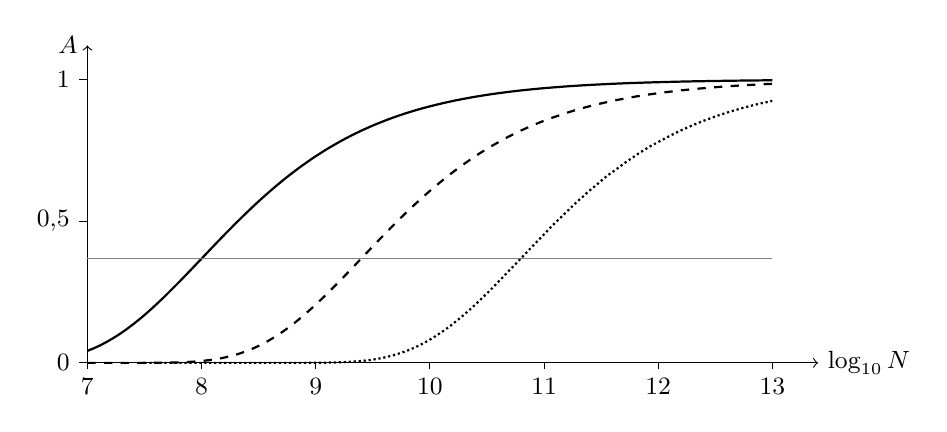
\begin{tikzpicture}[x=1.45cm,y=3.6cm,font=\small]
  \draw[->] (7,0)--(13.4,0) node[right] {$\log_{10}N$};
  \draw[->] (7,0)--(7,1.12) node[left] {$A$};
  \foreach \t in {7,8,...,13} \draw (\t,0)--(\t,-0.02) node[below] {\t};
  \foreach \t in {0,0.5,1} \draw (7,\t)--(6.93,\t) node[left] {\pgfmathprintnumber[use comma]{\t}};
  \draw[thick,domain=7:13,samples=120,smooth] plot (\x,{exp(-1*10^(-(\x-8)/2))});
  \draw[thick,dashed,domain=7:13,samples=120,smooth] plot (\x,{exp(-5*10^(-(\x-8)/2))});
  \draw[thick,densely dotted,domain=7.5:13,samples=120,smooth] plot (\x,{exp(-25*10^(-(\x-8)/2))});
  \draw[gray] (7,0.3679)--(13,0.3679);
\end{tikzpicture}
\caption{Exactitud exacta $A(N)=\exp\bigl(-k(10^{8}/N)^{1/2}\bigr)$ de la \cref{prop:gompertz} para respuestas de $k=1$ (continua), $k=5$ (discontinua) y $k=25$ (punteada) tokens. La línea gris marca $A=1/e$; los puntos de inflexión están en $\log_{10}N_0=8$, $9{,}40$ y $10{,}80$.}
\label{fig:gompertz}
\end{figure}

\begin{observacion}[El debate sigue abierto]
El argumento explica muchas discontinuidades observadas, y Schaeffer \emph{et al.}\ las hacen desaparecer cambiando la métrica o aumentando la resolución estadística~\cite{schaeffer}. No demuestra que no existan cambios cualitativos con la escala: muestra que una curva brusca en una métrica de todo o nada no es, por sí sola, prueba de ellos. Lo que sí está claro es que la pérdida de preentrenamiento es predecible y el rendimiento en una tarea concreta lo es mucho menos.
\end{observacion}

\section{El coste del contexto largo}

La ventana de contexto ha crecido de $2048$ tokens en GPT-3~\cite{brown} a 128K ($131\,072$) en Llama~3~\cite{llama3}; el informe de Gemini~1.5 describe ventanas de millones de tokens, con recuperación casi perfecta hasta al menos $10$ millones, y cita $200\,000$ tokens para Claude~3.0~\cite{gemini15}. Hay tres obstáculos.

\subsection*{Cómputo de la atención}

Por el módulo~14 (tema~6), una pasada hacia delante cuesta por token unos $2N+4L\nctx d$ FLOP, donde $L$ es el número de bloques y $d$ la dimensión del modelo. El segundo término procede de los productos $QK\T$ y $AV$ y crece linealmente con el contexto; sobre una secuencia completa, el coste de la atención crece como $\nctx^{2}$. Pasar de $4096$ a $10^{6}$ tokens multiplica ese término total por $(10^{6}/4096)^{2}\approx 59\,600$.

\begin{ejemplo}\label{ej:atencion-larga}
Para LLaMA-2~7B ($N=6{,}738\cdot 10^{9}$, $L=32$, $d=4096$), el término de atención por token vale $4\cdot 32\cdot 4096\cdot\nctx$. Con $\nctx=4096$ es $2{,}15\cdot 10^{9}$, el $13{,}7\,\%$ del total; con $32\,768$, $1{,}72\cdot 10^{10}$, el $56{,}0\,\%$; con $131\,072$, $6{,}87\cdot 10^{10}$, el $83{,}6\,\%$. A partir de unos $25\,700$ tokens, la atención cuesta más que todas las matrices de pesos juntas. FlashAttention (módulo~17) reduce el tráfico de memoria, pero no el número de operaciones.
\end{ejemplo}

\subsection*{Memoria de la caché KV}

\begin{proposicion}[Tamaño de la caché KV]\label{prop:kv}
Un Transformer de $L$ bloques con $h_{kv}$ cabezas de claves y valores de dimensión $d_k$, que almacena cada número con $\beta_b$ bytes, necesita para una secuencia de $n$ tokens una caché de
\[
M_{KV}=2\,L\,n\,h_{kv}\,d_k\,\beta_b\ \text{bytes}.
\]
\end{proposicion}

\begin{proof}
En cada bloque y para cada token previo se guardan un vector de claves y uno de valores por cabeza, cada uno de $d_k$ números: $2h_{kv}d_k$ números por token y bloque. Se multiplica por $L$ bloques, $n$ tokens y $\beta_b$ bytes por número.
\end{proof}

Para LLaMA-2~7B, con atención multicabeza estándar ($h_{kv}=32$, $d_k=128$) en bf16 ($\beta_b=2$), son $2\cdot 32\cdot 4096\cdot 2=524\,288$ bytes, $0{,}5$ MiB por token: $2$ GiB con $4096$ tokens y $64$ GiB con $131\,072$, más que la memoria de una GPU de $40$ GiB para una sola secuencia. La atención con consultas agrupadas (GQA, módulo~18) reduce $h_{kv}$: con $8$ cabezas de claves y valores, la caché se divide por~$4$. La caché domina el coste de la inferencia con contexto largo (módulo~19).

\section{Posiciones no vistas: interpolación de RoPE}

En RoPE (módulo~14, tema~4), el par de coordenadas $i$ de la consulta y la clave en la posición $m$ se rota un ángulo $m\theta_i$, con $\theta_i=\text{base}^{-2i/d_k}$ para $i=0,\dots,d_k/2-1$, y el producto escalar resultante depende solo de la diferencia de posiciones. Un modelo entrenado con contexto $L_{\mathrm{tr}}$ solo ha visto ángulos en $[0,L_{\mathrm{tr}}\theta_i)$. Para las frecuencias bajas, ese intervalo es una fracción pequeña de una vuelta, y las posiciones $m\ge L_{\mathrm{tr}}$ producen ángulos que el modelo nunca ha visto.

\begin{definicion}[Interpolación de posiciones; Chen \emph{et al.}~\cite{chenpi}]
Sea $L'>L_{\mathrm{tr}}$ el nuevo contexto. La \emph{interpolación de posiciones} sustituye la posición $m$ por $m\,L_{\mathrm{tr}}/L'$ en todas las rotaciones de RoPE, y se ajusta brevemente el modelo con secuencias de longitud $L'$.
\end{definicion}

\begin{proposicion}\label{prop:pi}
Con interpolación de posiciones, para toda posición $0\le m<L'$ y toda frecuencia $i$, el ángulo de rotación está en $[0,L_{\mathrm{tr}}\theta_i)$, el rango visto en el entrenamiento. El producto escalar rotado entre las posiciones $m$ y $n$ sigue dependiendo solo de $m-n$, ahora a través de $(m-n)L_{\mathrm{tr}}/L'$.
\end{proposicion}

\begin{proof}
El ángulo es $\theta_i\,mL_{\mathrm{tr}}/L'$, y $0\le mL_{\mathrm{tr}}/L'<L'L_{\mathrm{tr}}/L'=L_{\mathrm{tr}}$. Para la segunda afirmación, RoPE aplicado a posiciones reales $\mu$ y $\nu$ da un producto escalar que depende solo de $\mu-\nu$ (módulo~14, tema~4); con $\mu=mL_{\mathrm{tr}}/L'$ y $\nu=nL_{\mathrm{tr}}/L'$, $\mu-\nu=(m-n)L_{\mathrm{tr}}/L'$.
\end{proof}

\begin{ejemplo}\label{ej:pi}
Con base $10^{4}$ y $d_k=128$, la frecuencia más baja es $\theta_{63}=10^{-4\cdot 126/128}=1{,}155\cdot 10^{-4}$ rad por posición, con una longitud de onda de $2\pi/\theta_{63}\approx 54\,400$ posiciones. Con $L_{\mathrm{tr}}=2048$, el modelo solo ha visto ángulos hasta $0{,}237$ rad en esa frecuencia; en la posición $32\,768$ el ángulo sería $3{,}78$ rad, nunca visto. Con interpolación, el máximo sigue siendo $0{,}237$. Chen \emph{et al.}\ ampliaron así modelos LLaMA de $7\cdot 10^{9}$ a $65\cdot 10^{9}$ parámetros hasta $32\,768$ tokens con unos $1000$ pasos de ajuste, y obtuvieron una cota del error de la interpolación unas $600$ veces menor que la de la extrapolación~\cite{chenpi}.
\end{ejemplo}

El precio es la resolución: dos posiciones contiguas quedan a $L_{\mathrm{tr}}/L'$ de distancia en lugar de~$1$. Las variantes posteriores reparten el reescalado entre frecuencias (YaRN~\cite{yarn}) o aumentan la base de RoPE; Llama~3 usa base $500\,000$~\cite[§3.2]{llama3}.

\section{La receta habitual y sus límites}

Como el coste de la atención crece con el contexto, casi todo el preentrenamiento se hace con secuencias cortas y se añade una fase final con documentos largos. Llama~3 amplió su ventana de 8K a 128K tokens en seis etapas, con unos $800\,000$ millones de tokens en total~\cite[§3.4.2]{llama3}. Aceptar un contexto largo no equivale a usarlo bien: Liu \emph{et al.}~\cite{liu} observaron que los modelos aprovechan peor la información situada en el centro de un contexto largo que la situada al principio o al final.

\begin{lecturas}
\item Wei \emph{et al.}~\cite{wei} y Schaeffer, Miranda y Koyejo~\cite{schaeffer}.
\item Stanford CS324~\cite{cs324}, clase «Capabilities».
\item Bertsekas y Tsitsiklis~\cite{bt}, §1.5 «Independence» (ensayos independientes).
\item Chen \emph{et al.}~\cite{chenpi}, interpolación de posiciones; Peng \emph{et al.}~\cite{yarn}, YaRN.
\item Dubey \emph{et al.}~\cite{llama3}, §3.4.2 (preentrenamiento con contexto largo); Liu \emph{et al.}~\cite{liu}.
\end{lecturas}

\section*{Ejercicios del tema 6}
\addcontentsline{toc}{section}{Ejercicios del tema 6}

\begin{ejercicio}{1}{eje:6-escepticismo}
Un equipo afirma: «la capacidad~X aparece de golpe a partir de $10^{10}$ parámetros». Enumere tres comprobaciones que haría antes de aceptarlo y justifique cada una.
\end{ejercicio}

\begin{ejercicio}{2}{eje:6-todo-nada}
Una tarea exige generar exactamente una respuesta de $k$ tokens, y el modelo acierta cada token con probabilidad $p$, de forma independiente. (a) ¿Qué $p$ hace falta para una exactitud del $50\,\%$ con $k=10$? ¿Y con $k=20$? (b) Con $k=10$, ¿por qué factor se multiplica la exactitud al pasar de $p=0{,}8$ a $p=0{,}9$? (c) ¿Cuánto cambia, en el mismo paso, el número esperado de tokens correctos?
\fuente{adaptado de Bertsekas y Tsitsiklis~\cite{bt}, §1.5 (probabilidad de que tengan éxito todos los ensayos independientes de una serie).}
\end{ejercicio}

\begin{ejercicio}{2}{eje:6-atencion}
LLaMA~13B tiene $N\approx 1{,}3\cdot 10^{10}$ parámetros, $L=40$ bloques y $d=5120$. (a) ¿A partir de qué contexto el término de atención por token, $4L\nctx d$, supera a $2N$? (b) ¿Qué fracción del coste por token de la pasada hacia delante corresponde a la atención con $\nctx=8192$ y con $\nctx=131\,072$?
\end{ejercicio}

\begin{ejercicio}{2}{eje:6-kv}
Para el modelo del \cref{eje:6-atencion}, con $40$ cabezas de dimensión $d_k=128$ y caché en bf16: (a) calcule la caché KV por token; (b) calcule la caché de una secuencia de $32\,768$ tokens y la de un lote de $8$ secuencias; (c) ¿cuánto ocuparía la de una secuencia si el modelo usara GQA con $8$ cabezas de claves y valores?
\end{ejercicio}

\begin{ejercicio}{3}{eje:6-gompertz}
Con las hipótesis de la \cref{prop:gompertz}, $N_1=10^{8}$ y $\theta=1/2$: (a) calcule $A(N)$ para $k=5$ y $N=10^{8}$, $10^{9}$, $10^{10}$ y $10^{11}$; (b) halle el punto de inflexión para $k=1$, $5$ y $25$ y demuestre que multiplicar $k$ por $\lambda$ desplaza el umbral en $(\log_{10}\lambda)/\theta$ órdenes de magnitud; (c) demuestre que la pendiente máxima de $A$ respecto de $\ln N$ vale $\theta/e$, independiente de $k$, e interprete el resultado.
\end{ejercicio}

\begin{ejercicio}{3}{eje:6-pi}
Un modelo con RoPE (base $10^{4}$, $d_k=128$) se entrenó con $L_{\mathrm{tr}}=4096$ y se quiere ampliar a $L'=32\,768$. (a) Calcule el ángulo máximo visto en el entrenamiento para la frecuencia más baja y el que se alcanzaría sin interpolar. (b) Demuestre que con interpolación de posiciones todos los ángulos quedan en el rango visto. (c) Como alternativa, se aumenta la base: halle la base $b'$ con la que el ángulo máximo de la frecuencia más baja en $L'$ coincide con el del entrenamiento, y demuestre que con esa base las demás frecuencias $i\ge 1$ también giran menos que con la base original.
\end{ejercicio}


\appendix
% =====================================================================
\chapter{Soluciones de los ejercicios}
\label{ap:soluciones}
% =====================================================================

Cada solución se presenta en cinco partes: datos, planteamiento, desarrollo, resultado y comprobación. En los pasos intermedios se redondea a cuatro cifras significativas salvo que se indique otra cosa. Cuando un logaritmo se multiplica después por un exponente grande o se eleva a una potencia, se conservan cinco decimales, porque un error en la cuarta cifra de $\log_{10}N$ se nota en la tercera cifra de $N$. Todas las cifras se han comprobado con un programa en Python.

% ---------------------------------------------------------------------
\section{Tema 1}

\begin{solucion}{eje:1-sesgo}
\datos clasificador entrenado con páginas citadas desde la Wikipedia en inglés como positivos; rastreo multilingüe.
\planteamiento el clasificador aprende a reconocer lo que se parece a sus positivos; todo lo que difiere de ellos por razones ajenas a la calidad recibe puntuación baja.
\pasos
\begin{enumerate}[label=\arabic*.]
  \item Texto en otros idiomas, sobre todo los que tienen pocas páginas citadas en la Wikipedia inglesa: el clasificador confunde «distinto del inglés enciclopédico» con «de baja calidad».
  \item Registros informales y variedades dialectales (foros, conversación, literatura popular), útiles para un modelo de lenguaje general y ausentes del estilo enciclopédico.
  \item Consecuencia: el modelo resultante ve menos de esas variedades y las modeliza peor; su perplejidad sobre ellas es mayor y sus respuestas se sesgan hacia un registro y una cultura concretos.
  \item Medidas: aplicar el clasificador por idioma, con positivos de referencia de cada idioma; fijar el umbral por idioma o por dominio; y auditar muestras de lo descartado.
\end{enumerate}
\resultado \textbf{se descartan injustificadamente el texto en idiomas con pocos recursos y los registros informales o dialectales; el modelo hereda ese sesgo. Se mitiga con clasificadores y umbrales por idioma y con auditoría de lo descartado.}
\comprobacion la observación del \cref{tema:1} sobre la calidad como elección describe exactamente este mecanismo.
\end{solucion}

\begin{solucion}{eje:1-gopher}
\datos la tabla de cuatro documentos y las cuatro reglas de la \cref{def:gopher}.
\planteamiento calcular por documento la longitud media de palabra, la fracción de líneas con «...» y la fracción de palabras con letra; basta que falle una regla para descartarlo.
\pasos
\begin{enumerate}[label=\arabic*.]
  \item A: $40<50$ palabras, \textbf{falla} la regla~(i). El resto pasaría: $200/40=5{,}0$; $0/4=0$; $38/40=0{,}95$.
  \item B: $1200$ palabras, bien. Media $5640/1200=4{,}7$, bien. Líneas con «...»: $24/60=0{,}40>0{,}30$, \textbf{falla}. Letras: $1170/1200=0{,}975$.
  \item C: $800$ palabras; media $4160/800=5{,}2$; «...» $6/50=0{,}12\le 0{,}30$; letras $720/800=0{,}90\ge 0{,}80$. \textbf{Pasa}.
  \item D: $3000$ palabras; media $13\,500/3000=4{,}5$; «...» $5/100=0{,}05$; letras $2250/3000=0{,}75<0{,}80$, \textbf{falla}.
\end{enumerate}
\resultado \textbf{solo pasa C.} A es demasiado corto, B parece un listado de fragmentos truncados y D tiene demasiadas «palabras» sin letras (tablas, precios, códigos).
\comprobacion cada documento descartado falla exactamente una regla y con margen claro ($40$ frente a $50$; $0{,}40$ frente a $0{,}30$; $0{,}75$ frente a $0{,}80$): ningún resultado depende del redondeo.
\end{solucion}

\begin{solucion}{eje:1-mezcla}
\datos $D=10^{12}$. Web: $U=8\cdot 10^{11}$, $w=0{,}60$. Código: $2\cdot 10^{11}$, $0{,}25$. Libros: $5\cdot 10^{10}$, $0{,}10$. Ciencia: $10^{10}$, $0{,}05$.
\planteamiento $e_i=w_iD/U_i$ (\cref{def:mezcla}); más de unas $4$ épocas rinde poco (\cref{tema:5}).
\pasos
\begin{enumerate}[label=\arabic*.]
  \item Web: $0{,}60\cdot 10^{12}=6\cdot 10^{11}$ tokens vistos; $6\cdot 10^{11}/8\cdot 10^{11}=0{,}75$ épocas.
  \item Código: $2{,}5\cdot 10^{11}/2\cdot 10^{11}=1{,}25$ épocas.
  \item Libros: $10^{11}/5\cdot 10^{10}=2$ épocas.
  \item Ciencia: $5\cdot 10^{10}/10^{10}=5$ épocas.
  \item Ajuste: con $w=0{,}04$, la ciencia queda en $4\cdot 10^{10}/10^{10}=4$ épocas; el $0{,}01$ sobrante pasa a la web, que sube a $0{,}61\cdot 10^{12}/8\cdot 10^{11}=0{,}7625$ épocas.
\end{enumerate}
\resultado \textbf{web $0{,}75$; código $1{,}25$; libros $2$; ciencia $5$ épocas. Preocupa la ciencia ($5>4$); bajar su peso a $0{,}04$ y pasar $0{,}01$ a la web la deja en $4$.}
\comprobacion los pesos suman $0{,}60+0{,}25+0{,}10+0{,}05=1$ y los tokens vistos, $6+2{,}5+1+0{,}5=10$ (en $10^{11}$), es decir, $10^{12}=D$.
\end{solucion}

\begin{solucion}{eje:1-ppl}
\datos $q(\text{de})=0{,}4$, $q(\text{la})=0{,}3$, $q(\text{casa})=0{,}2$, $q(\text{oferta})=0{,}1$; documentos A, B y C de cuatro palabras; umbral $\PPL\le 4$.
\planteamiento $\PPL_q(x)=\bigl(\prod_tq(x_t)\bigr)^{-1/T}$ con $T=4$; para A, comparar $\ln\PPL$ con $H(\hat p)+D(\hat p\,\|\,q)$.
\pasos
\begin{enumerate}[label=\arabic*.]
  \item A: $\prod q=0{,}3\cdot 0{,}2\cdot 0{,}4\cdot 0{,}3=0{,}0072$; $\ln 0{,}0072=-4{,}9337$; $\ln\PPL=4{,}9337/4=1{,}2334$; $\PPL=e^{1{,}2334}=3{,}433$.
  \item B: $\prod q=0{,}1^{3}\cdot 0{,}2=0{,}0002$; $\ln\PPL=8{,}5172/4=2{,}1293$; $\PPL=8{,}409$.
  \item C: $\prod q=0{,}4^{4}$; $\PPL=1/0{,}4=2{,}5$.
  \item Con umbral~$4$ se conservan A y C, y se descarta B.
  \item Comprobación de la \cref{prop:ppl-kl} para A: $\hat p=(\text{de}:1/4,\ \text{la}:1/2,\ \text{casa}:1/4)$. $H(\hat p)=-\bigl(\tfrac14\ln\tfrac14+\tfrac12\ln\tfrac12+\tfrac14\ln\tfrac14\bigr)=1{,}0397$. $D(\hat p\,\|\,q)=\tfrac14\ln\tfrac{0{,}25}{0{,}4}+\tfrac12\ln\tfrac{0{,}5}{0{,}3}+\tfrac14\ln\tfrac{0{,}25}{0{,}2}=-0{,}1175+0{,}2554+0{,}0558=0{,}1937$. Suma: $1{,}2334$.
\end{enumerate}
\resultado \textbf{$\PPL(\text{A})=3{,}433$, $\PPL(\text{B})=8{,}409$, $\PPL(\text{C})=2{,}5$; pasan A y C.} El documento degenerado C obtiene la mejor puntuación, como predice el \cref{cor:repeticion}.
\comprobacion $1/q_{\max}=1/0{,}4=2{,}5$ es la cota inferior del \cref{cor:repeticion}, y la alcanza exactamente C; $H(\hat p)+D(\hat p\,\|\,q)=1{,}2334=\ln 3{,}433$.
\end{solucion}

\begin{solucion}{eje:1-fermi}
\datos $2500$ archivos en $1{,}5$ h por máquina; $100\,000$ archivos por volcado; $96$ volcados.
\planteamiento el filtrado es paralelo por archivos: el tiempo es proporcional al número de archivos e inversamente proporcional al número de máquinas.
\pasos
\begin{enumerate}[label=\arabic*.]
  \item (a) $100\,000/2500=40$ lotes; $40\cdot 1{,}5=60$ horas en una máquina.
  \item (b) $60/2=30$ máquinas.
  \item (c) $96\cdot 60=5760$ horas-máquina.
\end{enumerate}
\resultado \textbf{(a) $60$ h; (b) $30$ máquinas; (c) $5760$ horas-máquina.}
\comprobacion $30$ máquinas $\times\,2$ h $=60$ horas-máquina, el coste de un volcado; el orden de magnitud explica por qué la práctica de CS336 insiste en paralelizar~\cite[§4]{cs336a4}.
\end{solucion}

\begin{solucion}{eje:1-minmax}
\datos $D$ fijo; fuentes con $U_i$ tokens únicos; $e_i=w_iD/U_i$; tabla del \cref{ej:llama-mezcla}.
\planteamiento acotar inferiormente $\max_ie_i$ sumando las desigualdades $e_i\le\max_je_j$, y estudiar cuándo se alcanza la cota.
\pasos
\begin{enumerate}[label=\arabic*.]
  \item Sea $e=\max_ie_i$. Para todo $i$, $w_iD/U_i\le e$, es decir, $w_i\le eU_i/D$.
  \item Sumando y usando $\sum_iw_i=1$: $1\le e\sum_iU_i/D$, luego $e\ge D/\sum_iU_i$ para toda mezcla.
  \item La mezcla proporcional $w_i=U_i/\sum_jU_j$ da $e_i=D/\sum_jU_j$ para todo $i$: alcanza la cota y es óptima.
  \item Unicidad: si una mezcla alcanza $e=D/\sum_jU_j$, la suma del paso~2 es una igualdad, $\sum_iw_i=\sum_ieU_i/D$, y como cada sumando cumple $w_i\le eU_i/D$, todas las desigualdades son igualdades: $w_i=U_i/\sum_jU_j$.
  \item LLaMA: $\sum_iU_i=852{,}7+198{,}1+98{,}4+25{,}7+28{,}3+33{,}0+27{,}2=1263{,}4$ (en $10^{9}$). El mínimo es $1400/1263{,}4=1{,}108$ épocas.
\end{enumerate}
\resultado \textbf{la mezcla proporcional es la única que minimiza $\max_ie_i$, con valor $D/\sum_iU_i$; para LLaMA, $1{,}108$ épocas, frente a las $2{,}45$ que sus autores eligieron para Wikipedia.}
\comprobacion la elección de LLaMA no minimiza la repetición: sobremuestrea a propósito las fuentes pequeñas y valiosas, aceptando hasta $2{,}45$ épocas, por debajo del límite de unas $4$ del \cref{tema:5}.
\end{solucion}

% ---------------------------------------------------------------------
\section{Tema 2}

\begin{solucion}{eje:2-porque}
\datos dos corpus del mismo tamaño en tokens, uno con muchos duplicados y otro deduplicado.
\planteamiento comparar cuánta información nueva aporta cada token y qué hace el modelo con el texto que ve muchas veces.
\pasos
\begin{enumerate}[label=\arabic*.]
  \item \emph{Cómputo malgastado.} Un token duplicado no aporta información nueva: la entropía cruzada sobre él ya se redujo la primera vez. Con $C\approx 6ND$ fijo, el corpus efectivo es menor que su tamaño nominal.
  \item \emph{Memorización.} Lo repetido cientos de veces se aprende literalmente y puede regurgitarse, incluidos datos personales o protegidos~\cite{lee}.
  \item Además, \emph{contaminación}: si los duplicados cruzan la frontera entre entrenamiento y evaluación, las métricas se inflan.
\end{enumerate}
\resultado \textbf{(i) desperdicio de cómputo en información repetida; (ii) memorización literal (y, además, contaminación de la evaluación).}
\comprobacion caso límite: un corpus formado por un único documento repetido un millón de veces tiene el mismo tamaño en tokens, pero solo permite aprender ese documento.
\end{solucion}

\begin{solucion}{eje:2-conjuntos}
\datos $S_1=\{a,b,c,d\}$, $S_2=\{b,c,e\}$, $S_3=\{a,c,e,f\}$.
\planteamiento $J=\abs{X\cap Y}/\abs{X\cup Y}$ con $\abs{X\cup Y}=\abs X+\abs Y-\abs{X\cap Y}$.
\pasos
\begin{enumerate}[label=\arabic*.]
  \item $S_1,S_2$: intersección $\{b,c\}$; unión $4+3-2=5$; $J=2/5=0{,}4$.
  \item $S_1,S_3$: intersección $\{a,c\}$; unión $4+4-2=6$; $J=2/6=1/3$.
  \item $S_2,S_3$: intersección $\{c,e\}$; unión $3+4-2=5$; $J=2/5=0{,}4$.
\end{enumerate}
\resultado \textbf{$J(S_1,S_2)=0{,}4$; $J(S_1,S_3)=1/3\approx 0{,}333$; $J(S_2,S_3)=0{,}4$. Empatan $S_1$--$S_2$ y $S_2$--$S_3$.}
\comprobacion las tres intersecciones tienen $2$ elementos; el par con mayor unión, $S_1$--$S_3$, debe tener la menor similitud, y así es.
\end{solucion}

\begin{solucion}{eje:2-luna}
\datos A~=~«la luna brilla sobre el mar», B~=~«la luna brilla sobre el río»; $k=2$.
\planteamiento un texto de $T$ palabras tiene $T-1$ shingles de $2$ palabras; $J=\abs{A\cap B}/\abs{A\cup B}$.
\pasos
\begin{enumerate}[label=\arabic*.]
  \item A: $\{$la luna, luna brilla, brilla sobre, sobre el, el mar$\}$, $5$ shingles.
  \item B: $\{$la luna, luna brilla, brilla sobre, sobre el, el río$\}$, $5$ shingles.
  \item Intersección: los cuatro primeros, $\abs{A\cap B}=4$. Unión: $5+5-4=6$.
  \item $J=4/6=2/3$.
\end{enumerate}
\resultado \textbf{$J=2/3\approx 0{,}667$.}
\comprobacion solo cambia la última palabra, que aparece en un único shingle de cada frase: cada conjunto pierde $1$ de sus $5$ elementos y gana otro distinto. La fracción compartida de cada conjunto es $4/5$, pero la unión tiene $6>5$ elementos, de modo que $J<4/5$.
\end{solucion}

\begin{solucion}{eje:2-firmas}
\datos $S_1=\{0,2,5\}$, $S_2=\{1,2,3\}$, $S_3=\{0,3,5\}$; $h_1$, $h_2$, $h_3$ del enunciado.
\planteamiento una función es permutación del universo si toma los $6$ valores distintos; la firma es $(\min h_1,\min h_2,\min h_3)$ sobre cada conjunto; la similitud estimada es la fracción de coordenadas iguales.
\pasos
\begin{enumerate}[label=\arabic*.]
  \item Valores en $x=0,\dots,5$: $h_1=(1,2,3,4,5,0)$, permutación; $h_2=(1,0,5,4,3,2)$, permutación ($5$ y $6$ son primos entre sí); $h_3=(3,5,1,3,5,1)$, no lo es ($2$ y $6$ comparten el factor~$2$).
  \item $S_1=\{0,2,5\}$: $\min(1,3,0)=0$; $\min(1,5,2)=1$; $\min(3,1,1)=1$. Firma $(0,1,1)$.
  \item $S_2=\{1,2,3\}$: $\min(2,3,4)=2$; $\min(0,5,4)=0$; $\min(5,1,3)=1$. Firma $(2,0,1)$.
  \item $S_3=\{0,3,5\}$: $\min(1,4,0)=0$; $\min(1,4,2)=1$; $\min(3,3,1)=1$. Firma $(0,1,1)$.
  \item Similitudes reales: $J(S_1,S_2)=1/5=0{,}2$; $J(S_1,S_3)=2/4=0{,}5$; $J(S_2,S_3)=1/5=0{,}2$.
  \item Estimadas con las tres funciones: $S_1$--$S_2$ coinciden solo en $h_3$, $1/3$; $S_1$--$S_3$ en las tres, $1$; $S_2$--$S_3$ solo en $h_3$, $1/3$. Solo con $h_1$ y $h_2$: $0$, $1$ y $0$.
\end{enumerate}
\resultado \textbf{(a) $h_1$ y $h_2$ son permutaciones; $h_3$ no. (b) $\sig(S_1)=(0,1,1)$, $\sig(S_2)=(2,0,1)$, $\sig(S_3)=(0,1,1)$. (c) Reales: $0{,}2$; $0{,}5$; $0{,}2$. Estimadas: $1/3$; $1$; $1/3$.} Con tan pocas funciones el error es grande, y $h_3$, que no es permutación, coincide más de la cuenta.
\comprobacion por el \cref{cor:estimador}, con $J=0{,}5$ y $n=3$ la desviación típica es $\sqrt{0{,}25/3}=0{,}29$: estimar~$1$ está a menos de dos desviaciones típicas y es compatible con el azar.
\end{solucion}

\begin{solucion}{eje:2-lsh}
\datos $r=4$, $b=25$; $s=0{,}3$ y $s=0{,}85$.
\planteamiento $P(s)=1-(1-s^{r})^{b}$ (\cref{prop:curva-s}); para elevar a $25$, $x^{25}=e^{25\ln x}$.
\pasos
\begin{enumerate}[label=\arabic*.]
  \item $s=0{,}3$: $s^{4}=0{,}0081$; $\ln(0{,}9919)=-0{,}008133$; $25\cdot(-0{,}008133)=-0{,}2033$; $e^{-0{,}2033}=0{,}8160$; $P=0{,}1840$.
  \item $s=0{,}85$: $0{,}85^{4}=0{,}5220$; $\ln 0{,}4780=-0{,}7382$; $25\cdot(-0{,}7382)=-18{,}45$; $e^{-18{,}45}=9{,}7\cdot 10^{-9}$; $P=1-9{,}7\cdot 10^{-9}$.
  \item Umbral aproximado: $(1/25)^{1/4}=\sqrt{\sqrt{0{,}04}}=\sqrt{0{,}2}=0{,}4472$.
  \item Inflexión exacta: $\bigl((r-1)/(rb-1)\bigr)^{1/r}=(3/99)^{1/4}=0{,}4172$.
\end{enumerate}
\resultado \textbf{$P(0{,}3)\approx 0{,}184$; $P(0{,}85)\approx 1-10^{-8}$; umbral aproximado $0{,}447$; inflexión $0{,}417$.}
\comprobacion $0{,}3<0{,}417<0{,}85$, así que la curva debe dar una probabilidad baja en el primer caso y casi~$1$ en el segundo. Con $r=4$, pequeño, la aproximación $(1/b)^{1/r}$ se separa algo de la inflexión exacta, como prevé la \cref{prop:curva-s}.
\end{solucion}

\begin{solucion}{eje:2-curvas}
\datos $(r,b)=(3,10)$, $(6,20)$, $(5,50)$; $s=0{,}2$, $0{,}5$, $0{,}8$.
\planteamiento $P(s)=1-(1-s^{r})^{b}$; de $P=1/2$ se despeja $s_{1/2}=(1-2^{-1/b})^{1/r}$.
\pasos
\begin{enumerate}[label=\arabic*.]
  \item $(3,10)$. $s=0{,}2$: $s^{3}=0{,}008$; $0{,}992^{10}=0{,}9228$; $P=0{,}0772$. $s=0{,}5$: $0{,}875^{10}=0{,}2631$; $P=0{,}7369$. $s=0{,}8$: $0{,}488^{10}=7{,}66\cdot 10^{-4}$; $P=0{,}9992$.
  \item $(6,20)$. $s=0{,}2$: $s^{6}=6{,}4\cdot 10^{-5}$; $P=0{,}0013$. $s=0{,}5$: $s^{6}=0{,}015625$; $0{,}984375^{20}=0{,}7298$; $P=0{,}2702$. $s=0{,}8$: $s^{6}=0{,}2621$; $0{,}7379^{20}=0{,}00229$; $P=0{,}9977$.
  \item $(5,50)$. $s=0{,}2$: $s^{5}=3{,}2\cdot 10^{-4}$; $0{,}99968^{50}=0{,}9841$; $P=0{,}0159$. $s=0{,}5$: $0{,}96875^{50}=0{,}2044$; $P=0{,}7956$. $s=0{,}8$: $0{,}6723^{50}=2{,}4\cdot 10^{-9}$; $P\approx 1$.
  \item $s_{1/2}$ para $(3,10)$: $2^{-1/10}=0{,}9330$; $0{,}0670^{1/3}=0{,}4061$, frente a $(1/10)^{1/3}=0{,}4642$.
  \item Para $(6,20)$: $2^{-1/20}=0{,}9659$; $0{,}0341^{1/6}=0{,}5694$, frente a $(1/20)^{1/6}=0{,}6070$.
  \item Para $(5,50)$: $2^{-1/50}=0{,}9862$; $0{,}0138^{1/5}=0{,}4244$, frente a $(1/50)^{1/5}=0{,}4573$.
\end{enumerate}
\resultado \textbf{(a) $(0{,}077;\ 0{,}737;\ 0{,}999)$ para $(3,10)$; $(0{,}001;\ 0{,}270;\ 0{,}998)$ para $(6,20)$; $(0{,}016;\ 0{,}796;\ 1{,}000)$ para $(5,50)$. (b) $s_{1/2}=0{,}406$; $0{,}569$; $0{,}424$, frente a $0{,}464$; $0{,}607$; $0{,}457$: la aproximación sobrestima el punto del $50\,\%$ entre $0{,}03$ y $0{,}06$.}
\comprobacion $0{,}4061^{3}=0{,}0670$ y $0{,}9330^{10}=0{,}500$. Además, $(6,20)$, con más filas por banda, es la curva más exigente: da la menor $P$ en $s=0{,}5$.
\end{solucion}

\begin{solucion}{eje:2-varianza}
\datos $\Var(\hat J)=J(1-J)/n$ (\cref{cor:estimador}).
\planteamiento acotar $J(1-J)$ en $[0,1]$; despejar $n$; aplicar Chebyshev, $\PP(\abs{X-\E X}\ge\varepsilon)\le\Var(X)/\varepsilon^{2}$ (módulo~5).
\pasos
\begin{enumerate}[label=\arabic*.]
  \item (a) $J(1-J)=\tfrac14-(J-\tfrac12)^{2}\le\tfrac14$, con igualdad en $J=1/2$. Luego $\sqrt{\Var(\hat J)}\le\sqrt{1/(4n)}=1/(2\sqrt n)$.
  \item (b) Para todo par: $1/(2\sqrt n)\le 0{,}05\iff\sqrt n\ge 10\iff n\ge 100$.
  \item Con $J=0{,}8$: $J(1-J)=0{,}16$; $0{,}16/n\le 0{,}0025\iff n\ge 64$.
  \item (c) $\PP(\abs{\hat J-J}\ge 0{,}1)\le\dfrac{J(1-J)}{100\cdot 0{,}01}\le\dfrac{0{,}25}{1}=0{,}25$.
\end{enumerate}
\resultado \textbf{(a) $\sigma\le 1/(2\sqrt n)$; (b) $n=100$ en general y $n=64$ si $J=0{,}8$; (c) probabilidad a lo sumo $0{,}25$.}
\comprobacion con $n=100$ y $J=1/2$, el error de $0{,}1$ son dos desviaciones típicas; la aproximación normal daría una probabilidad de unos $0{,}05$, compatible con la cota de Chebyshev, que es más conservadora.
\end{solucion}

% ---------------------------------------------------------------------
\section{Tema 3}

\begin{solucion}{eje:3-recta}
\datos $L=kN^{-\alpha}$; $\alpha=0{,}076$.
\planteamiento tomar logaritmos con $\log(xy)=\log x+\log y$ y $\log x^{a}=a\log x$ (\cref{prop:loglog}).
\pasos
\begin{enumerate}[label=\arabic*.]
  \item $\log L=\log k+\log N^{-\alpha}=\log k-\alpha\log N$.
  \item Con $u=\log N$ y $v=\log L$: $v=\log k-\alpha u$, una recta de pendiente $-\alpha$ y ordenada $\log k$.
  \item Multiplicar $N$ por $10$ aumenta $u=\log_{10}N$ en $1$, luego $v$ baja $\alpha=0{,}076$.
\end{enumerate}
\resultado \textbf{la ley es una recta de pendiente $-\alpha$; la pendiente es el cambio de $\log L$ por cada unidad de $\log N$. Con $\alpha=0{,}076$, $\log_{10}L$ baja $0{,}076$ por cada factor~$10$ en $N$.}
\comprobacion $10^{-0{,}076}=0{,}8395$: $L$ se multiplica por $0{,}84$, como en el \cref{ej:kaplan}.
\end{solucion}

\begin{solucion}{eje:3-computo}
\datos $N=1{,}3\cdot 10^{9}$; $D=2{,}6\cdot 10^{10}$; $1$ PF-día $=8{,}64\cdot 10^{19}$ FLOP.
\planteamiento $C\approx 6ND$; tokens por parámetro $=D/N$.
\pasos
\begin{enumerate}[label=\arabic*.]
  \item $6N=7{,}8\cdot 10^{9}$.
  \item $C=7{,}8\cdot 10^{9}\cdot 2{,}6\cdot 10^{10}=20{,}28\cdot 10^{19}=2{,}028\cdot 10^{20}$ FLOP.
  \item En PF-días: $2{,}028\cdot 10^{20}/8{,}64\cdot 10^{19}=2{,}347$.
  \item $D/N=2{,}6\cdot 10^{10}/1{,}3\cdot 10^{9}=20$.
\end{enumerate}
\resultado \textbf{$C=2{,}028\cdot 10^{20}$ FLOP $\approx 2{,}35$ PF-días; $20$ tokens por parámetro.}
\comprobacion con la \cref{prop:regla20}, $\sqrt{C/120}=\sqrt{1{,}69\cdot 10^{18}}=1{,}3\cdot 10^{9}$: se recupera el $N$ de partida.
\end{solucion}

\begin{solucion}{eje:3-datos}
\datos $L(D)=(5{,}4\cdot 10^{13}/D)^{0{,}095}$; $D=10^{9}$ y $10^{11}$.
\planteamiento $x^{0{,}095}=10^{0{,}095\log_{10}x}$.
\pasos
\begin{enumerate}[label=\arabic*.]
  \item $D=10^{9}$: $x=5{,}4\cdot 10^{4}$; $\log_{10}x=4{,}73239$; $0{,}095\cdot 4{,}73239=0{,}44958$; $L=10^{0{,}44958}=2{,}816$.
  \item $D=10^{11}$: $x=540$; $\log_{10}x=2{,}73239$; $0{,}095\cdot 2{,}73239=0{,}25958$; $L=10^{0{,}25958}=1{,}818$.
  \item Factor por cada factor~$10$: $10^{-0{,}095}=0{,}8035$.
\end{enumerate}
\resultado \textbf{$L(10^{9})\approx 2{,}816$ nats; $L(10^{11})\approx 1{,}818$ nats; cada factor~$10$ en $D$ multiplica $L$ por $0{,}804$.}
\comprobacion de $10^{9}$ a $10^{11}$ hay dos factores~$10$: $2{,}816\cdot 0{,}8035^{2}=2{,}816\cdot 0{,}6456=1{,}818$.
\end{solucion}

\begin{solucion}{eje:3-ajuste}
\datos configuraciones $(4,256)$, $(8,512)$, $(16,1024)$ con $L=4{,}20$, $3{,}62$, $3{,}12$; $N=12n_{\mathrm{layer}}d_{\mathrm{model}}^{2}$.
\planteamiento calcular $u_j=\log_{10}N_j$ y $v_j=\log_{10}L_j$ y aplicar la \cref{def:ajuste}.
\pasos
\begin{enumerate}[label=\arabic*.]
  \item (a) $N_1=12\cdot 4\cdot 65\,536=3\,145\,728$; $N_2=12\cdot 8\cdot 262\,144=25\,165\,824$; $N_3=12\cdot 16\cdot 1\,048\,576=201\,326\,592$. Cada uno es $8$ veces el anterior.
  \item $u=(6{,}49772;\ 7{,}40081;\ 8{,}30390)$, equiespaciados con paso $\log_{10}8=0{,}90309$; $\bar u=7{,}40081$.
  \item $v=(0{,}62325;\ 0{,}55871;\ 0{,}49415)$; $\bar v=0{,}55870$.
  \item Numerador: $(-0{,}90309)(0{,}06455)+0+(0{,}90309)(-0{,}06455)=-0{,}11658$. Denominador: $2\cdot 0{,}90309^{2}=1{,}63114$.
  \item $b_1=-0{,}11658/1{,}63114=-0{,}07147$; $b_0=0{,}55870+0{,}07147\cdot 7{,}40081=1{,}08767$.
  \item (c) $N=12\cdot 32\cdot 2048^{2}=1\,610\,612\,736$; $\log_{10}N=9{,}20700$; $\log_{10}\hat L=1{,}08767-0{,}07147\cdot 9{,}20700=0{,}42963$; $\hat L=2{,}689$.
\end{enumerate}
\resultado \textbf{(a) $N=3{,}15\cdot 10^{6}$, $2{,}52\cdot 10^{7}$, $2{,}01\cdot 10^{8}$; (b) $\hat L=10^{1{,}0877}N^{-0{,}0715}$, exponente $\hat\alpha=0{,}0715$; (c) $\hat L\approx 2{,}69$ nats para $N=1{,}61\cdot 10^{9}$.} La predicción extrapola un orden de magnitud con solo tres puntos y supone que los hiperparámetros (tasa de aprendizaje, lote, tokens) se ajustan bien en todos los tamaños; sin varias semillas no hay barras de error.
\comprobacion la recta ajustada reproduce los datos: $10^{1{,}08767-0{,}07147\cdot 6{,}49772}=4{,}200$, $3{,}620$ y $3{,}120$. El exponente es del orden del $\alpha_N=0{,}076$ de Kaplan \emph{et al.}
\end{solucion}

\begin{solucion}{eje:3-sobreajuste}
\datos $L(N,D)$ de~\eqref{eq:kaplan-nd}; $L(N)=(N_c/N)^{\alpha_N}$; $\alpha_N=0{,}076$; $\alpha_D=0{,}095$ o $0{,}103$.
\planteamiento sacar factor común $(N_c/N)^{\alpha_N/\alpha_D}$ dentro del corchete.
\pasos
\begin{enumerate}[label=\arabic*.]
  \item Sea $\rho=\alpha_N/\alpha_D$. El corchete es $(N_c/N)^{\rho}\bigl(1+(N/N_c)^{\rho}D_c/D\bigr)$.
  \item Elevando a $\alpha_D$ y usando $\rho\alpha_D=\alpha_N$:
  \[
  L(N,D)=\Bigl(\frac{N_c}{N}\Bigr)^{\rho\alpha_D}\Bigl(1+\Bigl(\frac{N}{N_c}\Bigr)^{\rho}\frac{D_c}{D}\Bigr)^{\alpha_D}=L(N)\Bigl(1+\frac{N^{\rho}D_c}{N_c^{\rho}D}\Bigr)^{\alpha_D},
  \]
  que es la igualdad~(a).
  \item (b) El cociente depende de $N$ y $D$ solo a través de $z=N^{\rho}/D$, y es creciente en $z$. Para mantenerlo constante al crecer $N$, $z$ debe mantenerse constante: $D\propto N^{\rho}=N^{\alpha_N/\alpha_D}$.
  \item (c) Con $\alpha_D=0{,}095$: $\rho=0{,}076/0{,}095=0{,}80$. Con $\alpha_D=0{,}103$: $\rho=0{,}076/0{,}103=0{,}738$.
\end{enumerate}
\resultado \textbf{$L(N,D)/L(N)=\bigl(1+(N/N_c)^{\alpha_N/\alpha_D}D_c/D\bigr)^{\alpha_D}$; $D$ debe crecer como $N^{\alpha_N/\alpha_D}$, con exponente $0{,}80$ o $0{,}74$ según el ajuste.} El segundo valor es el de la regla $D\gtrsim 5\cdot 10^{3}N^{0{,}74}$.
\comprobacion cuando $D\to\infty$, el cociente tiende a $1$, de acuerdo con la \cref{prop:limites}; el crecimiento sublineal ($\rho<1$) significa que los modelos grandes necesitan menos datos por parámetro para no sobreajustar.
\end{solucion}

\begin{solucion}{eje:3-invariancia}
\datos $b_1=\sum(u_j-\bar u)(v_j-\bar v)/\sum(u_j-\bar u)^{2}$, $b_0=\bar v-b_1\bar u$, $\hat\alpha=-b_1$.
\planteamiento cada transformación cambia $u$ o $v$ de forma afín; ver cómo cambian las desviaciones respecto de la media.
\pasos
\begin{enumerate}[label=\arabic*.]
  \item (a) Cambiar de base multiplica todos los logaritmos por la misma constante $\kappa_0>0$: $u'_j=\kappa_0u_j$, $v'_j=\kappa_0v_j$. Las desviaciones se multiplican por $\kappa_0$; numerador y denominador de $b_1$ por $\kappa_0^{2}$, y $b_1'=b_1$. La ordenada pasa a $b_0'=\kappa_0b_0$.
  \item (b) $N'=\kappa N$ da $u'_j=u_j+\log\kappa$: $\bar u'=\bar u+\log\kappa$ y $u'_j-\bar u'=u_j-\bar u$. Luego $b_1'=b_1$ y $b_0'=\bar v-b_1(\bar u+\log\kappa)=b_0-b_1\log\kappa$.
  \item (c) $L'=cL$ da $v'_j=v_j+\log c$, con $v'_j-\bar v'=v_j-\bar v$: $b_1'=b_1$ y $b_0'=b_0+\log c$. De nats a bits, $c=1/\ln 2$.
\end{enumerate}
\resultado \textbf{$\hat\alpha$ es invariante en los tres casos; cambia la ordenada: $b_0'=\kappa_0b_0$, $b_0'=b_0-b_1\log\kappa$ y $b_0'=b_0+\log c$, respectivamente.}
\comprobacion es coherente con la \cref{prop:escala}: el exponente es la única característica de una ley de potencia que no depende de las unidades, y la constante absorbe todos los cambios de escala.
\end{solucion}

% ---------------------------------------------------------------------
\section{Tema 4}

\begin{solucion}{eje:4-vf}
\planteamiento recordar los exponentes de $\Nopt$ en cada trabajo y el papel de $E$.
\pasos
\begin{enumerate}[label=(\alph*)]
  \item \textbf{Verdadera.} Kaplan \emph{et al.}\ obtienen $\Nopt\propto C^{0{,}73}$ y $D\propto C^{0{,}27}$: el exponente del modelo es casi el triple que el de los datos.
  \item \textbf{Falsa.} A cómputo fijo hay un tamaño óptimo (\cref{teo:chinchilla}); Gopher era demasiado grande para su presupuesto y Chinchilla, cuatro veces menor, obtiene menos pérdida: $1{,}937$ frente a $1{,}993$ (\cref{ej:gopher-chinchilla}).
  \item \textbf{Falsa.} $E=1{,}69$ no depende de $N$ ni de $D$: es la entropía del texto, y $L\to E$ cuando $N,D\to\infty$.
\end{enumerate}
\resultado \textbf{(a) V; (b) F; (c) F.}
\comprobacion en (c), con $N=D=10^{30}$ los términos de error valen $2{,}6\cdot 10^{-8}$ y $1{,}6\cdot 10^{-6}$, y $L\approx 1{,}69$.
\end{solucion}

\begin{solucion}{eje:4-regla20}
\datos $C=10^{23}$; $D=20N$.
\planteamiento por la \cref{prop:regla20}, $N=\sqrt{C/120}$.
\pasos
\begin{enumerate}[label=\arabic*.]
  \item $N^{2}=10^{23}/120=8{,}333\cdot 10^{20}$.
  \item $N=\sqrt{8{,}333}\cdot 10^{10}=2{,}887\cdot 10^{10}$.
  \item $D=20\cdot 2{,}887\cdot 10^{10}=5{,}774\cdot 10^{11}$.
\end{enumerate}
\resultado \textbf{$N\approx 2{,}89\cdot 10^{10}$ parámetros y $D\approx 5{,}77\cdot 10^{11}$ tokens.}
\comprobacion $6\cdot 2{,}887\cdot 10^{10}\cdot 5{,}774\cdot 10^{11}=1{,}000\cdot 10^{23}$.
\end{solucion}

\begin{solucion}{eje:4-optimo}
\datos $E=1{,}69$, $A=406{,}4$, $\alpha=0{,}34$, $B=410{,}7$, $\beta=0{,}28$; $C=10^{22}$.
\planteamiento \cref{teo:chinchilla}: $\Nopt=G(C/6)^{a}$, $\Dopt=(C/6)/\Nopt$; después $L=E+A\Nopt^{-\alpha}+B\Dopt^{-\beta}$.
\pasos
\begin{enumerate}[label=\arabic*.]
  \item $a=0{,}28/0{,}62=0{,}45161$; $1/(\alpha+\beta)=1{,}6129$.
  \item $\alpha A=138{,}18$; $\beta B=115{,}00$; cociente $1{,}20157$; $\ln 1{,}20157=0{,}18363$; $G=e^{1{,}6129\cdot 0{,}18363}=e^{0{,}29618}=1{,}3447$.
  \item $C/6=1{,}6667\cdot 10^{21}$; $\log_{10}(C/6)=21{,}22185$; $(C/6)^{a}=10^{0{,}45161\cdot 21{,}22185}=10^{9{,}58406}=3{,}8376\cdot 10^{9}$.
  \item $\Nopt=1{,}3447\cdot 3{,}8376\cdot 10^{9}=5{,}160\cdot 10^{9}$.
  \item $\Dopt=1{,}6667\cdot 10^{21}/5{,}160\cdot 10^{9}=3{,}230\cdot 10^{11}$; $\Dopt/\Nopt=62{,}6$.
  \item $\log_{10}\Nopt=9{,}71265$; $\Nopt^{0{,}34}=10^{3{,}30230}=2006$; $T_N=406{,}4/2006=0{,}2026$.
  \item $\log_{10}\Dopt=11{,}50920$; $\Dopt^{0{,}28}=10^{3{,}22258}=1669{,}5$; $T_D=410{,}7/1669{,}5=0{,}2460$.
  \item $L=1{,}69+0{,}2026+0{,}2460=2{,}1386$.
  \item Regla de~20: $N=\sqrt{10^{22}/120}=9{,}129\cdot 10^{9}$ y $D=1{,}826\cdot 10^{11}$. Términos de error: $406{,}4/10^{0{,}34\cdot 9{,}96042}=406{,}4/2435=0{,}1669$ y $410{,}7/10^{0{,}28\cdot 11{,}26150}=410{,}7/1423=0{,}2886$. Pérdida: $L=2{,}1455$.
\end{enumerate}
\resultado \textbf{$\Nopt\approx 5{,}16\cdot 10^{9}$; $\Dopt\approx 3{,}23\cdot 10^{11}$; $\Dopt/\Nopt\approx 63$; $L\approx 2{,}1386$ nats. La regla de~20 da $N\approx 9{,}13\cdot 10^{9}$, $D\approx 1{,}83\cdot 10^{11}$ y $L\approx 2{,}1455$: solo $0{,}007$ nats peor.}
\comprobacion (i) $6\cdot 5{,}160\cdot 10^{9}\cdot 3{,}230\cdot 10^{11}=1{,}000\cdot 10^{22}$. (ii) Por el \cref{cor:equilibrio}, $T_D/T_N$ debe valer $\alpha/\beta=1{,}214$: $0{,}2460/0{,}2026=1{,}214$.
\end{solucion}

\begin{solucion}{eje:4-plano}
\datos $T_N=0{,}2026$, $T_D=0{,}2460$, $\alpha=0{,}34$, $\beta=0{,}28$; factores $\lambda=4$ y $\lambda=1/4$.
\planteamiento \cref{prop:plano} con $\delta=\ln\lambda=\pm 1{,}3863$.
\pasos
\begin{enumerate}[label=\arabic*.]
  \item Coeficiente cuadrático: $\tfrac12(\alpha^{2}T_N+\beta^{2}T_D)=\tfrac12(0{,}1156\cdot 0{,}2026+0{,}0784\cdot 0{,}2460)=0{,}02135$; con $\delta^{2}=1{,}9218$, aproximación $0{,}0410$ en ambos casos.
  \item $\lambda=4$: $e^{-0{,}34\cdot 1{,}3863}=e^{-0{,}4713}=0{,}6242$ y $e^{0{,}28\cdot 1{,}3863}=e^{0{,}3882}=1{,}4743$. $\Delta=0{,}2026\cdot(-0{,}3758)+0{,}2460\cdot 0{,}4743=-0{,}07614+0{,}11668=0{,}0405$.
  \item $\lambda=1/4$: $e^{0{,}4713}=1{,}6021$ y $e^{-0{,}3882}=0{,}6783$. $\Delta=0{,}2026\cdot 0{,}6021+0{,}2460\cdot(-0{,}3217)=0{,}12198-0{,}07914=0{,}0429$.
  \item Asimetría: el término cúbico del desarrollo es $\tfrac16(-\alpha^{3}T_N+\beta^{3}T_D)\delta^{3}$, con $-\alpha^{3}T_N+\beta^{3}T_D=-0{,}00796+0{,}00540=-0{,}00256<0$; resta en $\delta>0$ y suma en $\delta<0$.
\end{enumerate}
\resultado \textbf{exceso exacto $0{,}0405$ nats con $4\Nopt$ y $0{,}0429$ con $\Nopt/4$; la aproximación cuadrática da $0{,}0410$ en ambos.} Equivocarse por exceso en el tamaño cuesta algo menos que por defecto, porque $\alpha>\beta$.
\comprobacion $\delta^{3}/6\cdot(-0{,}00256)=\mp 0{,}00114$, y $0{,}0410-0{,}0011=0{,}0399$ y $0{,}0410+0{,}0011=0{,}0421$ se acercan a los valores exactos; el resto lo aportan los términos de orden~4.
\end{solucion}

\begin{solucion}{eje:4-factor4}
\datos $\Nopt=G(C/6)^{a}$, $a=\beta/(\alpha+\beta)$; $\Dopt=(C/6)/\Nopt$; $\alpha=0{,}34$, $\beta=0{,}28$.
\planteamiento dividir la fórmula en $4C$ entre la fórmula en $C$; $G$ y el factor $1/6$ se cancelan.
\pasos
\begin{enumerate}[label=\arabic*.]
  \item $\Nopt(4C)/\Nopt(C)=G(4C/6)^{a}/\bigl(G(C/6)^{a}\bigr)=4^{a}$.
  \item $\Dopt=G^{-1}(C/6)^{1-a}$, porque $x/x^{a}=x^{1-a}$; del mismo modo, $\Dopt(4C)/\Dopt(C)=4^{1-a}$.
  \item $1-a=(\alpha+\beta-\beta)/(\alpha+\beta)=\alpha/(\alpha+\beta)$.
  \item $a=0{,}45161$ y $1-a=0{,}54839$; $\log_{10}4=0{,}60206$.
  \item $4^{0{,}45161}=10^{0{,}27190}=1{,}870$; $4^{0{,}54839}=10^{0{,}33017}=2{,}139$.
\end{enumerate}
\resultado \textbf{$\Nopt$ se multiplica por $4^{\beta/(\alpha+\beta)}\approx 1{,}870$ y $\Dopt$ por $4^{\alpha/(\alpha+\beta)}\approx 2{,}139$.}
\comprobacion $1{,}870\cdot 2{,}139=4{,}000$, como exige $6\Nopt\Dopt=C$.
\end{solucion}

\begin{solucion}{eje:4-perdida}
\datos $\Nopt=Gc^{a}$, $\Dopt=G^{-1}c^{b}$, $c=C/6$; valores de Chinchilla; del \cref{eje:4-optimo}, $T_N+T_D=0{,}4486$ en $10^{22}$.
\planteamiento seguir la demostración del \cref{cor:perdida} conservando las constantes.
\pasos
\begin{enumerate}[label=\arabic*.]
  \item $A\Nopt^{-\alpha}=AG^{-\alpha}c^{-\gamma}$ y $B\Dopt^{-\beta}=BG^{\beta}c^{-\gamma}$, con $\gamma=\alpha a=\beta b=\alpha\beta/(\alpha+\beta)$.
  \item $L^{*}-E=(AG^{-\alpha}+BG^{\beta})c^{-\gamma}=(AG^{-\alpha}+BG^{\beta})\,6^{\gamma}\,C^{-\gamma}$, luego $K=(AG^{-\alpha}+BG^{\beta})\,6^{\gamma}$.
  \item $\gamma=0{,}0952/0{,}62=0{,}15355$. $G^{-\alpha}=1{,}3447^{-0{,}34}=0{,}9042$ y $G^{\beta}=1{,}3447^{0{,}28}=1{,}0865$; $AG^{-\alpha}=367{,}47$ y $BG^{\beta}=446{,}21$; suma $813{,}68$; $6^{\gamma}=1{,}3167$; $K=1071{,}4$.
  \item En $10^{22}$: $C^{-\gamma}=10^{-22\cdot 0{,}15355}=4{,}187\cdot 10^{-4}$, y $K C^{-\gamma}=0{,}4486$.
  \item De $10^{22}$ a $10^{24}$: factor $100^{-\gamma}=10^{-0{,}30710}=0{,}4931$; exceso $0{,}4486\cdot 0{,}4931=0{,}2212$.
  \item Directamente en $10^{24}$: $\Nopt=4{,}130\cdot 10^{10}$, $\Dopt=4{,}036\cdot 10^{12}$, $T_N=0{,}0999$, $T_D=0{,}1213$; suma $0{,}2212$.
\end{enumerate}
\resultado \textbf{$K=(AG^{-\alpha}+BG^{\beta})6^{\gamma}\approx 1071$, $\gamma\approx 0{,}154$. Con $100$ veces más cómputo, el exceso pasa de $0{,}449$ a $0{,}221$ nats (factor $0{,}493$).}
\comprobacion el cálculo directo del paso~6 coincide con la ley del paso~5, y el valor de $K C^{-\gamma}$ en $10^{22}$ reproduce la suma $T_N+T_D$ del \cref{eje:4-optimo}.
\end{solucion}

\begin{solucion}{eje:4-gp}
\datos $f(N,D)=AN^{-\alpha}+BD^{-\beta}$; restricción $6ND\le C$; $T_N=0{,}2026$, $T_D=0{,}2460$, $\gamma=0{,}15355$ en $C=10^{22}$.
\planteamiento cambio de variables logarítmico~\cite[§4.5]{bv}; condiciones KKT~\cite[§5.5]{bv}; comparación con el \cref{cor:perdida}.
\pasos
\begin{enumerate}[label=\arabic*.]
  \item (a) Con $N=e^{u}$, $D=e^{v}$: minimizar $\tilde f(u,v)=Ae^{-\alpha u}+Be^{-\beta v}$ sujeto a $u+v-\ln(C/6)\le 0$. Cada sumando es la exponencial, convexa y creciente, de una función afín, luego convexo; la suma es convexa. La restricción es afín. El problema es convexo.
  \item (b) Si en un punto factible la restricción no fuera activa, $u+v<\ln(C/6)$, aumentar $u$ ligeramente seguiría siendo factible y reduciría estrictamente $Ae^{-\alpha u}$. Luego en el óptimo $u+v=\ln(C/6)$, es decir, $6ND=C$.
  \item (c) En las variables originales, KKT: $\nabla f+\mu\nabla(6ND-C)=0$, $\mu\ge 0$, $\mu(6ND-C)=0$. Las componentes dan $-\alpha AN^{-\alpha-1}+6\mu D=0$ y $-\beta BD^{-\beta-1}+6\mu N=0$, que son las del \cref{teo:chinchilla} con $\lambda=\mu$. De la primera, $\mu=\alpha AN^{-\alpha}/(6ND)=\alpha T_N/C>0$, compatible con la restricción activa. Como el problema transformado es convexo, estas condiciones son suficientes.
  \item Numéricamente, $\mu C=\alpha T_N=0{,}34\cdot 0{,}2026=0{,}0689$.
  \item (d) Por el \cref{cor:perdida}, $dL^{*}/d\ln C=-\gamma KC^{-\gamma}=-\gamma(T_N+T_D)$. Como $T_D=(\alpha/\beta)T_N$, $\gamma(T_N+T_D)=\gamma T_N(\alpha+\beta)/\beta=\alpha T_N=\mu C$. Luego $dL^{*}/d\ln C=-\mu C$, es decir, $dL^{*}/dC=-\mu$.
  \item Con los datos: $\gamma(T_N+T_D)=0{,}15355\cdot 0{,}4486=0{,}0689$.
\end{enumerate}
\resultado \textbf{el problema es convexo en $(\ln N,\ln D)$; la restricción es activa; el punto del \cref{teo:chinchilla} satisface KKT con $\mu=\alpha T_N/C>0$, y $\mu$ es el ritmo al que baja la pérdida óptima por unidad de cómputo: $dL^{*}/d\ln C=-0{,}0689$ nats en $10^{22}$ FLOP.}
\comprobacion duplicar el cómputo ($\Delta\ln C=0{,}693$) debería reducir la pérdida en unos $0{,}0689\cdot 0{,}693=0{,}048$ nats; el \cref{cor:perdida} da $0{,}4486\cdot(1-2^{-0{,}15355})=0{,}4486\cdot 0{,}1009=0{,}0453$, del mismo orden (la diferencia procede de la curvatura).
\end{solucion}

% ---------------------------------------------------------------------
\section{Tema 5}

\begin{solucion}{eje:5-sobreentreno}
\datos coste de entrenamiento $6ND$; coste de inferencia $2N$ por token servido.
\planteamiento comparar costes totales (\cref{prop:amortizacion}).
\pasos
\begin{enumerate}[label=\arabic*.]
  \item El óptimo de Chinchilla minimiza solo $6ND$ para una pérdida dada. Un modelo menor necesita más tokens para igualar la pérdida, y su entrenamiento cuesta más (\cref{prop:sobrecoste}).
  \item Pero cada token servido cuesta $2N$: un modelo la mitad de grande ahorra la mitad del cómputo de inferencia, para siempre. Con millones de usuarios, $T_{\mathrm{inf}}$ supera enseguida el umbral $T^{*}$ de la \cref{prop:amortizacion}.
  \item Además, un modelo menor requiere menos memoria y responde con menos latencia.
  \item El óptimo de Chinchilla es preferible cuando el modelo se usará poco (un experimento, un prototipo, un modelo de investigación) o cuando el cuello de botella es el cómputo de entrenamiento disponible.
\end{enumerate}
\resultado \textbf{porque el coste total incluye $2N T_{\mathrm{inf}}$, que domina con mucha demanda; el óptimo de Chinchilla conviene cuando se servirán pocos tokens.}
\comprobacion en el \cref{ej:sobreentreno}, el sobrecoste se amortiza tras $1{,}1\cdot 10^{11}$ tokens: $10^{6}$ usuarios que generan $10^{5}$ tokens cada uno ya lo superan.
\end{solucion}

\begin{solucion}{eje:5-isoflop}
\datos la tabla de nueve entrenamientos en tres presupuestos.
\planteamiento mínimo de cada perfil; recta en $(\log_{10}C,\log_{10}\Nopt)$; $D=C/(6N)$.
\pasos
\begin{enumerate}[label=\arabic*.]
  \item Mínimos: $10^{18}\to 5\cdot 10^{7}$ ($3{,}85$); $10^{19}\to 1{,}6\cdot 10^{8}$ ($3{,}40$); $10^{20}\to 5\cdot 10^{8}$ ($3{,}01$).
  \item $x=18,19,20$; $y=7{,}69897;\ 8{,}20412;\ 8{,}69897$; $\bar x=19$; $\bar y=24{,}60206/3=8{,}20069$.
  \item Pendiente: numerador $(-1)(-0{,}50172)+0+(1)(0{,}49828)=1{,}00000$; denominador $2$; $a=0{,}5$.
  \item Ordenada: $b_0=8{,}20069-0{,}5\cdot 19=-1{,}29931$.
  \item $C=10^{23}$: $\log_{10}N=10{,}20069$; $N=1{,}587\cdot 10^{10}$; $D=10^{23}/(9{,}522\cdot 10^{10})=1{,}050\cdot 10^{12}$; $D/N=66{,}1$.
  \item $C=10^{24}$: $\log_{10}N=10{,}70069$; $N=5{,}020\cdot 10^{10}$; $D=3{,}320\cdot 10^{12}$; $D/N=66{,}1$.
\end{enumerate}
\resultado \textbf{$\Nopt\propto C^{0{,}5}$. En $10^{23}$: $N\approx 1{,}59\cdot 10^{10}$, $D\approx 1{,}05\cdot 10^{12}$; en $10^{24}$: $N\approx 5{,}02\cdot 10^{10}$, $D\approx 3{,}32\cdot 10^{12}$; unos $66$ tokens por parámetro, más que la regla de~20 en estos datos sintéticos.}
\comprobacion con $a=0{,}5$, $N$ y $D$ crecen como $\sqrt C$ y $D/N$ es constante: sale $66$ en ambos presupuestos; además, $6\cdot 1{,}587\cdot 10^{10}\cdot 1{,}050\cdot 10^{12}=1{,}000\cdot 10^{23}$.
\end{solucion}

\begin{solucion}{eje:5-vertice}
\datos $C=10^{19}$; $x=(8{,}0;\ 8{,}3;\ 8{,}6)$, $h=0{,}3$; $L=(3{,}47;\ 3{,}40;\ 3{,}43)$.
\planteamiento \cref{prop:vertice}; $D=C/(6N)$.
\pasos
\begin{enumerate}[label=\arabic*.]
  \item $\Delta_2=3{,}47-6{,}80+3{,}43=0{,}10>0$; $L_3-L_1=-0{,}04$.
  \item $x^{*}=8{,}3-0{,}3\cdot(-0{,}04)/(2\cdot 0{,}10)=8{,}3+0{,}06=8{,}36$; $\Nopt=10^{8{,}36}=2{,}291\cdot 10^{8}$.
  \item $L^{*}=3{,}40-0{,}0016/0{,}8=3{,}398$.
  \item $\Dopt=10^{19}/(6\cdot 2{,}291\cdot 10^{8})=7{,}275\cdot 10^{9}$; $\Dopt/\Nopt=31{,}8$.
  \item El criterio del mínimo observado daría $10^{8{,}3}=1{,}995\cdot 10^{8}$, un $13\,\%$ menos.
\end{enumerate}
\resultado \textbf{vértice en $\log_{10}N=8{,}36$: $\Nopt\approx 2{,}29\cdot 10^{8}$, $L^{*}\approx 3{,}398$, $\Dopt\approx 7{,}3\cdot 10^{9}$ ($32$ tokens por parámetro). El mínimo observado da $2{,}0\cdot 10^{8}$.}
\comprobacion la parábola $p(t)=3{,}40-0{,}02t+0{,}05t^{2}$ pasa por los tres puntos ($p(-1)=3{,}47$, $p(1)=3{,}43$) y su mínimo, en $t^{*}=0{,}2$, vale $3{,}40-0{,}004+0{,}002=3{,}398$. El vértice se desplaza hacia el lado de la pérdida menor ($L_3<L_1$).
\end{solucion}

\begin{solucion}{eje:5-repetir}
\datos $U=10^{11}$; $R^{*}=15{,}39$; entrenamientos de $4\cdot 10^{11}$ y $1{,}6\cdot 10^{12}$ tokens.
\planteamiento épocas $=D/U$; $R=$ épocas $-1$; $D'=U\bigl(1+R^{*}(1-e^{-R/R^{*}})\bigr)$.
\pasos
\begin{enumerate}[label=\arabic*.]
  \item Primer entrenamiento: $4$ épocas, $R=3$; $R/R^{*}=0{,}1949$; $1-e^{-0{,}1949}=0{,}1771$; $D'=10^{11}(1+15{,}39\cdot 0{,}1771)=3{,}726\cdot 10^{11}$; fracción $3{,}726/4=0{,}931$.
  \item Segundo: $16$ épocas, $R=15$; $R/R^{*}=0{,}9748$; $1-e^{-0{,}9748}=0{,}6227$; $D'=10^{11}(1+15{,}39\cdot 0{,}6227)=1{,}058\cdot 10^{12}$; fracción $1{,}058/1{,}6=0{,}661$.
  \item Máximo: $U(1+R^{*})=1{,}639\cdot 10^{12}$ (\cref{prop:efectivos}).
\end{enumerate}
\resultado \textbf{$D'=3{,}73\cdot 10^{11}$ ($93\,\%$ de lo procesado) con $4$ épocas y $D'=1{,}06\cdot 10^{12}$ ($66\,\%$) con $16$; el máximo alcanzable es $1{,}64\cdot 10^{12}$ tokens efectivos.}
\comprobacion cuadruplicar el entrenamiento de $4$ a $16$ épocas solo multiplica los datos efectivos por $1{,}058/0{,}3726=2{,}84$: el rendimiento marginal decrece, como exige la concavidad de la \cref{prop:efectivos}.
\end{solucion}

\begin{solucion}{eje:5-reto}
\datos $C=10^{22}$; del \cref{eje:4-optimo}, $N_1=5{,}1605\cdot 10^{9}$, $L_1=2{,}13861$; $N_2=N_1/2$; inferencia $2N$ por token.
\planteamiento despejar $D_2$ de $L(N_2,D_2)=L_1$; $C_2=6N_2D_2$; $T^{*}$ de la \cref{prop:amortizacion} con $6N_1D_1=C$. Se usan cinco cifras porque el exponente $1/0{,}28=3{,}571$ amplifica los errores.
\pasos
\begin{enumerate}[label=\arabic*.]
  \item $N_2=2{,}5802\cdot 10^{9}$; $\log_{10}N_2=9{,}41165$; $N_2^{0{,}34}=10^{3{,}19996}=1584{,}7$; $A/N_2^{\alpha}=0{,}25645$.
  \item $B/D_2^{\beta}=2{,}13861-1{,}69-0{,}25645=0{,}19216$.
  \item $D_2^{0{,}28}=410{,}7/0{,}19216=2137{,}3$; $\log_{10}D_2=3{,}32986/0{,}28=11{,}89236$; $D_2=7{,}803\cdot 10^{11}$.
  \item Tokens por parámetro: $7{,}803\cdot 10^{11}/2{,}5802\cdot 10^{9}=302$.
  \item $C_2=6\cdot 2{,}5802\cdot 10^{9}\cdot 7{,}803\cdot 10^{11}=1{,}208\cdot 10^{22}$; sobrecoste $2{,}08\cdot 10^{21}$ FLOP.
  \item Ahorro por token servido: $2(N_1-N_2)=5{,}160\cdot 10^{9}$ FLOP; $T^{*}=2{,}08\cdot 10^{21}/5{,}160\cdot 10^{9}=4{,}03\cdot 10^{11}$ tokens.
  \item \cref{prop:sobrecoste} con $\kappa=1/2$: $C_2/C=1{,}208$, igual que en el paso~5.
\end{enumerate}
\resultado \textbf{$D_2\approx 7{,}80\cdot 10^{11}$ tokens ($302$ por parámetro); el entrenamiento cuesta $1{,}208$ veces más ($+2{,}08\cdot 10^{21}$ FLOP) y se amortiza tras unos $4{,}0\cdot 10^{11}$ tokens de inferencia.}
\comprobacion sustituyendo, $1{,}69+0{,}25645+410{,}7/2137{,}3=1{,}69+0{,}25645+0{,}19216=2{,}13861=L_1$. El sobrecoste relativo es el mismo que a $10^{21}$ FLOP (\cref{ej:sobreentreno}), como predice la \cref{prop:sobrecoste}; el umbral de amortización, en cambio, escala con el presupuesto.
\end{solucion}

\begin{solucion}{eje:5-cota}
\datos $D'=U+UR^{*}(1-e^{-R/R^{*}})$, $R\ge 0$.
\planteamiento acotar $1-e^{-x}$ entre $x-x^{2}/2$ y $x$ para $x\ge 0$.
\pasos
\begin{enumerate}[label=\arabic*.]
  \item Sea $\psi(x)=x-(1-e^{-x})$. $\psi(0)=0$ y $\psi'(x)=1-e^{-x}\ge 0$: $1-e^{-x}\le x$.
  \item Sea $\chi(x)=(1-e^{-x})-x+x^{2}/2$. $\chi(0)=0$ y $\chi'(x)=e^{-x}-1+x\ge 0$ por el paso~1 aplicado a $e^{-x}\ge 1-x$: $1-e^{-x}\ge x-x^{2}/2$.
  \item Con $x=R/R^{*}$ y multiplicando por $UR^{*}>0$: $UR-UR^{2}/(2R^{*})\le UR^{*}(1-e^{-R/R^{*}})\le UR$. Sumando $U$ se obtiene la doble desigualdad.
  \item Dividiendo por $U(1+R)$: $1-D'/(U(1+R))\le R^{2}/\bigl(2R^{*}(1+R)\bigr)\le R/(2R^{*})$, porque $R/(1+R)\le 1$.
  \item Cuatro épocas ($R=3$): cota $3/(2\cdot 15{,}39)=0{,}0975$ (la intermedia, $9/(2\cdot 15{,}39\cdot 4)=0{,}0731$); valor exacto $1-0{,}9314=0{,}0686$.
\end{enumerate}
\resultado \textbf{$U(1+R)-UR^{2}/(2R^{*})\le D'\le U(1+R)$; la pérdida de valor es a lo sumo $R/(2R^{*})$: un $9{,}8\,\%$ con cuatro épocas, frente al $6{,}9\,\%$ exacto.}
\comprobacion con $R=3$, la cota inferior da $4-0{,}2924=3{,}708$ (en unidades de $U$), y el valor exacto, $3{,}726$, está entre ella y $4$.
\end{solucion}

% ---------------------------------------------------------------------
\section{Tema 6}

\begin{solucion}{eje:6-escepticismo}
\datos una afirmación de emergencia a partir de $10^{10}$ parámetros.
\planteamiento aplicar el argumento de la métrica (\cref{prop:gompertz}) y las precauciones experimentales habituales.
\pasos
\begin{enumerate}[label=\arabic*.]
  \item \emph{La métrica.} Si es exactitud exacta sobre respuestas de $k$ tokens, vale $p^{k}$: con $k=10$, pasar de $p=0{,}8$ a $0{,}95$ lleva la exactitud de $0{,}107$ a $0{,}599$. Hay que repetir la medida con una métrica continua (log-probabilidad de la respuesta correcta, distancia de edición). Si la curva es suave, el salto lo crea la métrica.
  \item \emph{La resolución.} Con tres o cuatro tamaños de modelo, cualquier curva en S parece un escalón. Hacen falta tamaños intermedios y varias semillas para estimar barras de error.
  \item \emph{La contaminación.} Un modelo mayor memoriza más; si la tarea aparece en el corpus, puede «aprobar» por haber visto las respuestas.
\end{enumerate}
\resultado \textbf{comprobaría la métrica (todo o nada frente a continua), la densidad de tamaños con su incertidumbre y la contaminación del corpus.}
\comprobacion con la tabla del \cref{tema:6}, pasar de $p=0{,}8$ a $0{,}9$ con $k=10$ multiplica la exactitud por $0{,}349/0{,}107\approx 3{,}3$, mientras que $p$ solo crece un $12{,}5\,\%$.
\end{solucion}

\begin{solucion}{eje:6-todo-nada}
\datos $k$ tokens independientes con probabilidad de acierto $p$.
\planteamiento exactitud $p^{k}$ (independencia); número esperado de aciertos $kp$ (esperanza de una binomial).
\pasos
\begin{enumerate}[label=\arabic*.]
  \item (a) $p^{10}=0{,}5\iff p=0{,}5^{1/10}=0{,}9330$. Con $k=20$: $p=0{,}5^{1/20}=0{,}9659$.
  \item (b) $0{,}9^{10}=0{,}3487$ y $0{,}8^{10}=0{,}1074$; cociente $(0{,}9/0{,}8)^{10}=1{,}125^{10}=3{,}247$.
  \item (c) $kp$ pasa de $8$ a $9$: un $12{,}5\,\%$ más, el mismo aumento relativo que $p$.
\end{enumerate}
\resultado \textbf{(a) $p\approx 0{,}933$ con $k=10$ y $p\approx 0{,}966$ con $k=20$; (b) la exactitud se multiplica por $3{,}25$; (c) los aciertos esperados crecen un $12{,}5\,\%$ (de $8$ a $9$).}
\comprobacion $0{,}9330^{10}=0{,}500$; la respuesta más larga exige una $p$ mayor para la misma exactitud, coherente con el desplazamiento del umbral de la \cref{prop:gompertz}.
\end{solucion}

\begin{solucion}{eje:6-atencion}
\datos $N=1{,}3\cdot 10^{10}$; $L=40$; $d=5120$.
\planteamiento coste por token $2N+4L\nctx d$ (módulo~14); umbral $n^{*}=N/(2Ld)$.
\pasos
\begin{enumerate}[label=\arabic*.]
  \item (a) $n^{*}=1{,}3\cdot 10^{10}/(2\cdot 40\cdot 5120)=1{,}3\cdot 10^{10}/409\,600=31\,738$ tokens.
  \item (b) $\nctx=8192$: $4\cdot 40\cdot 8192\cdot 5120=6{,}711\cdot 10^{9}$; $2N=2{,}6\cdot 10^{10}$; fracción $6{,}711/(26+6{,}711)=0{,}205$.
  \item $\nctx=131\,072$: $1{,}074\cdot 10^{11}$; fracción $1{,}074/(0{,}26+1{,}074)=0{,}805$.
\end{enumerate}
\resultado \textbf{(a) a partir de unos $31\,700$ tokens; (b) la atención es el $20{,}5\,\%$ del coste por token con $8192$ tokens y el $80{,}5\,\%$ con $131\,072$.}
\comprobacion el término de atención es lineal en $\nctx$: $131\,072/8192=16$ y $16\cdot 6{,}711\cdot 10^{9}=1{,}074\cdot 10^{11}$.
\end{solucion}

\begin{solucion}{eje:6-kv}
\datos $L=40$; $h_{kv}=40$, $d_k=128$ ($h_{kv}d_k=5120$); bf16, $\beta_b=2$.
\planteamiento \cref{prop:kv}; $1$ MiB $=2^{20}$ bytes y $1$ GiB $=2^{30}$ bytes.
\pasos
\begin{enumerate}[label=\arabic*.]
  \item (a) Por token: $2\cdot 40\cdot 5120\cdot 2=819\,200$ bytes $=0{,}78125$ MiB.
  \item (b) $32\,768$ tokens: $819\,200\cdot 32\,768=26\,843\,545\,600$ bytes $=25$ GiB. Lote de $8$: $200$ GiB.
  \item (c) Con $h_{kv}=8$, la caché se multiplica por $8/40=1/5$: $5$ GiB por secuencia.
\end{enumerate}
\resultado \textbf{(a) $0{,}78$ MiB por token; (b) $25$ GiB por secuencia y $200$ GiB por lote; (c) $5$ GiB con GQA de $8$ cabezas.}
\comprobacion $819\,200=0{,}78125\cdot 2^{20}$ y $0{,}78125\cdot 32\,768=25\,600$ MiB $=25$ GiB: la caché de una sola secuencia larga supera ya la mitad de una GPU de $40$ GiB.
\end{solucion}

\begin{solucion}{eje:6-gompertz}
\datos $\ell(N)=(10^{8}/N)^{1/2}$; $A(N)=e^{-k\ell(N)}$.
\planteamiento evaluar $A$; usar la \cref{prop:gompertz}~(ii) para la inflexión; derivar $A$ respecto de $x=\ln N$.
\pasos
\begin{enumerate}[label=\arabic*.]
  \item (a) $k=5$: $N=10^{8}$: $\ell=1$, $A=e^{-5}=0{,}0067$. $N=10^{9}$: $\ell=0{,}3162$, $A=e^{-1{,}581}=0{,}2057$. $N=10^{10}$: $\ell=0{,}1$, $A=e^{-0{,}5}=0{,}6065$. $N=10^{11}$: $\ell=0{,}0316$, $A=e^{-0{,}1581}=0{,}8538$.
  \item (b) $N_0=N_1k^{1/\theta}=10^{8}k^{2}$: $10^{8}$, $2{,}5\cdot 10^{9}$ y $6{,}25\cdot 10^{10}$ para $k=1$, $5$ y $25$ ($\log_{10}N_0=8$; $9{,}40$; $10{,}80$).
  \item Con $k\to\lambda k$: $\log_{10}N_0$ pasa de $\log_{10}N_1+(\log_{10}k)/\theta$ a $\log_{10}N_1+(\log_{10}k+\log_{10}\lambda)/\theta$: se desplaza $(\log_{10}\lambda)/\theta$ órdenes de magnitud. Con $\lambda=5$ y $\theta=1/2$, $2\log_{10}5=1{,}40$.
  \item (c) Por la demostración de la \cref{prop:gompertz}, $dA/dx=\theta ye^{-y}$ con $y=e^{-\theta(x-x_0)}>0$. La función $ye^{-y}$ alcanza su máximo, $e^{-1}$, en $y=1$; luego $\max dA/dx=\theta/e$, que no depende de $k$.
\end{enumerate}
\resultado \textbf{(a) $A=0{,}007$; $0{,}206$; $0{,}607$; $0{,}854$; (b) inflexiones en $10^{8}$, $2{,}5\cdot 10^{9}$ y $6{,}25\cdot 10^{10}$; el umbral se desplaza $(\log_{10}\lambda)/\theta$ órdenes de magnitud; (c) pendiente máxima $\theta/e$.} La «brusquedad» de la transición en escala logarítmica es la misma para cualquier longitud de respuesta: alargar la respuesta solo traslada la curva hacia modelos mayores.
\comprobacion en $N_0=2{,}5\cdot 10^{9}$ con $k=5$: $\ell=(1/25)^{1/2}=0{,}2$ y $A=e^{-1}=0{,}368$, como exige la \cref{prop:gompertz}; el valor cae entre los de $10^{9}$ y $10^{10}$ del apartado~(a).
\end{solucion}

\begin{solucion}{eje:6-pi}
\datos base $10^{4}$; $d_k=128$; $L_{\mathrm{tr}}=4096$; $L'=32\,768$.
\planteamiento frecuencia más baja $\theta_{63}=\text{base}^{-126/128}$; \cref{prop:pi}; para la base nueva, igualar $L'\theta'_{63}=L_{\mathrm{tr}}\theta_{63}$.
\pasos
\begin{enumerate}[label=\arabic*.]
  \item (a) $\theta_{63}=10^{-4\cdot 0{,}984375}=10^{-3{,}9375}=1{,}1548\cdot 10^{-4}$. Ángulo máximo en el entrenamiento: $4096\cdot 1{,}1548\cdot 10^{-4}=0{,}4730$ rad. Sin interpolar, en $L'$: $32\,768\cdot 1{,}1548\cdot 10^{-4}=3{,}784$ rad.
  \item (b) Con interpolación, la posición $m<L'$ se sustituye por $m/8$, y el ángulo es $\theta_i m/8<\theta_iL'/8=\theta_iL_{\mathrm{tr}}$, dentro del rango visto (\cref{prop:pi}).
  \item (c) Se busca $b'$ con $L'(b')^{-126/128}=L_{\mathrm{tr}}\,10^{-4\cdot 126/128}$, es decir, $(b'/10^{4})^{126/128}=L'/L_{\mathrm{tr}}=8$, de donde $b'=10^{4}\cdot 8^{128/126}=10^{4}\cdot 8{,}2685=82\,685$.
  \item Para $i\ge 1$, $\theta_i'=(b')^{-2i/d_k}<10^{-4\cdot 2i/d_k}=\theta_i$ porque $b'>10^{4}$ y el exponente $-2i/d_k$ es negativo: todas las frecuencias giran más despacio.
\end{enumerate}
\resultado \textbf{(a) $0{,}473$ rad en el entrenamiento frente a $3{,}78$ rad sin interpolar; (b) con interpolación ningún ángulo supera el rango visto; (c) $b'\approx 82\,700$, y con ella todas las frecuencias giran más despacio que con la base original.}
\comprobacion $32\,768\cdot 82\,685^{-126/128}=32\,768\cdot 1{,}4436\cdot 10^{-5}=0{,}4730$ rad, el máximo del entrenamiento. A diferencia de la interpolación, aumentar la base no comprime por igual todas las frecuencias: las altas, que ya daban muchas vueltas en el entrenamiento, cambian poco.
\end{solucion}


\backmatter
% =====================================================================
\begin{thebibliography}{99}
\addcontentsline{toc}{chapter}{Bibliografía}
\markboth{Bibliografía}{}
\small
\def\UrlBreaks{\do\/\do-}

\bibitem{bt}
D.~P. Bertsekas y J.~N. Tsitsiklis.
\newblock \emph{Introduction to Probability}, 2.ª ed.
\newblock Athena Scientific, 2008.
\newblock Texto del curso 6.041 del MIT. §1.5, «Independence».

\bibitem{besiroglu}
T.~Besiroglu, E.~Erdil, M.~Barnett y J.~You.
\newblock Chinchilla scaling: A replication attempt.
\newblock Prepublicación, 2024.
\newblock \url{https://arxiv.org/abs/2404.10102}

\bibitem{bv}
S.~Boyd y L.~Vandenberghe.
\newblock \emph{Convex Optimization}.
\newblock Cambridge University Press, 2004.
\newblock §4.5 «Geometric programming» y §5.5 «Optimality conditions».
\newblock \url{https://web.stanford.edu/~boyd/cvxbook/}

\bibitem{broder}
A.~Z. Broder.
\newblock On the resemblance and containment of documents.
\newblock En \emph{Proceedings of Compression and Complexity of Sequences}, IEEE, 1997.

\bibitem{brown}
T.~B. Brown \emph{et al.}
\newblock Language models are few-shot learners.
\newblock En \emph{Advances in Neural Information Processing Systems 33 (NeurIPS)}, 2020.
\newblock \url{https://arxiv.org/abs/2005.14165}

\bibitem{chenpi}
S.~Chen, S.~Wong, L.~Chen e Y.~Tian.
\newblock Extending context window of large language models via positional interpolation.
\newblock Prepublicación, 2023.
\newblock \url{https://arxiv.org/abs/2306.15595}

\bibitem{llama3}
A.~Dubey \emph{et al.} (Llama Team, Meta).
\newblock The Llama 3 herd of models.
\newblock Prepublicación, 2024.
\newblock \url{https://arxiv.org/abs/2407.21783}

\bibitem{gemini15}
Gemini Team, Google.
\newblock Gemini 1.5: Unlocking multimodal understanding across millions of tokens of context.
\newblock Informe técnico, 2024.
\newblock \url{https://arxiv.org/abs/2403.05530}

\bibitem{cs336a3}
T.~Hashimoto y P.~Liang.
\newblock CS336: Language Modeling from Scratch.
\newblock Stanford University, primavera de 2026. Práctica~3, «Scaling Laws», versión~26.0.5.
\newblock \url{https://github.com/stanford-cs336/assignment3-scaling}

\bibitem{cs336a4}
T.~Hashimoto y P.~Liang.
\newblock CS336: Language Modeling from Scratch.
\newblock Stanford University, primavera de 2026. Práctica~4, «Data: Filtering Language Modeling Data», versión~26.0.1.
\newblock \url{https://github.com/stanford-cs336/assignment4-data}

\bibitem{hoffmann}
J.~Hoffmann, S.~Borgeaud, A.~Mensch \emph{et al.}
\newblock Training compute-optimal large language models.
\newblock En \emph{Advances in Neural Information Processing Systems 35 (NeurIPS)}, 2022.
\newblock \url{https://arxiv.org/abs/2203.15556}

\bibitem{kaplan}
J.~Kaplan, S.~McCandlish, T.~Henighan, T.~B. Brown, B.~Chess, R.~Child, S.~Gray, A.~Radford, J.~Wu y D.~Amodei.
\newblock Scaling laws for neural language models.
\newblock Prepublicación, 2020.
\newblock \url{https://arxiv.org/abs/2001.08361}

\bibitem{lee}
K.~Lee, D.~Ippolito, A.~Nystrom, C.~Zhang, D.~Eck, C.~Callison-Burch y N.~Carlini.
\newblock Deduplicating training data makes language models better.
\newblock En \emph{Proceedings of ACL}, 2022.
\newblock \url{https://arxiv.org/abs/2107.06499}

\bibitem{cs246}
J.~Leskovec.
\newblock CS246: Mining Massive Data Sets.
\newblock Stanford University, invierno de 2026. Clases «Locality-Sensitive Hashing~I» y «Locality-Sensitive Hashing~II».
\newblock \url{https://web.stanford.edu/class/cs246/}

\bibitem{mmds}
J.~Leskovec, A.~Rajaraman y J.~D. Ullman.
\newblock \emph{Mining of Massive Datasets}, 3.ª ed.
\newblock Cambridge University Press, 2020.
\newblock Cap.~3, «Finding Similar Items».
\newblock \url{http://infolab.stanford.edu/~ullman/mmds/ch3n.pdf}

\bibitem{cs324}
P.~Liang, T.~Hashimoto y C.~Ré.
\newblock CS324: Large Language Models.
\newblock Stanford University, invierno de 2022. Notas de las clases «Capabilities», «Data» y «Scaling laws».
\newblock \url{https://stanford-cs324.github.io/winter2022/lectures/}

\bibitem{liu}
N.~F. Liu, K.~Lin, J.~Hewitt, A.~Paranjape, M.~Bevilacqua, F.~Petroni y P.~Liang.
\newblock Lost in the middle: How language models use long contexts.
\newblock \emph{Transactions of the Association for Computational Linguistics}, 12, 2024.
\newblock \url{https://arxiv.org/abs/2307.03172}

\bibitem{muennighoff}
N.~Muennighoff, A.~M. Rush, B.~Barak, T.~Le~Scao, A.~Piktus, N.~Tazi, S.~Pyysalo, T.~Wolf y C.~Raffel.
\newblock Scaling data-constrained language models.
\newblock En \emph{Advances in Neural Information Processing Systems 36 (NeurIPS)}, 2023.
\newblock \url{https://arxiv.org/abs/2305.16264}

\bibitem{refinedweb}
G.~Penedo \emph{et al.}
\newblock The RefinedWeb dataset for Falcon LLM: Outperforming curated corpora with web data, and web data only.
\newblock Prepublicación, 2023.
\newblock \url{https://arxiv.org/abs/2306.01116}

\bibitem{fineweb}
G.~Penedo, H.~Kydlíček, L.~Ben~Allal, A.~Lozhkov, M.~Mitchell, C.~Raffel, L.~Von~Werra y T.~Wolf.
\newblock The FineWeb datasets: Decanting the web for the finest text data at scale.
\newblock Prepublicación, 2024.
\newblock \url{https://arxiv.org/abs/2406.17557}

\bibitem{yarn}
B.~Peng, J.~Quesnelle, H.~Fan y E.~Shippole.
\newblock YaRN: Efficient context window extension of large language models.
\newblock Prepublicación, 2023.
\newblock \url{https://arxiv.org/abs/2309.00071}

\bibitem{rae}
J.~W. Rae \emph{et al.}
\newblock Scaling language models: Methods, analysis \& insights from training Gopher.
\newblock Prepublicación, 2021.
\newblock \url{https://arxiv.org/abs/2112.11446}

\bibitem{sardana}
N.~Sardana, J.~Portes, S.~Doubov y J.~Frankle.
\newblock Beyond Chinchilla-optimal: Accounting for inference in language model scaling laws.
\newblock Prepublicación, 2023.
\newblock \url{https://arxiv.org/abs/2401.00448}

\bibitem{schaeffer}
R.~Schaeffer, B.~Miranda y S.~Koyejo.
\newblock Are emergent abilities of large language models a mirage?
\newblock En \emph{Advances in Neural Information Processing Systems 36 (NeurIPS)}, 2023.
\newblock \url{https://arxiv.org/abs/2304.15004}

\bibitem{llama}
H.~Touvron \emph{et al.}
\newblock LLaMA: Open and efficient foundation language models.
\newblock Prepublicación, 2023.
\newblock \url{https://arxiv.org/abs/2302.13971}

\bibitem{llama2}
H.~Touvron \emph{et al.}
\newblock Llama 2: Open foundation and fine-tuned chat models.
\newblock Prepublicación, 2023.
\newblock \url{https://arxiv.org/abs/2307.09288}

\bibitem{wei}
J.~Wei, Y.~Tay, R.~Bommasani, C.~Raffel, B.~Zoph, S.~Borgeaud, D.~Yogatama, M.~Bosma, D.~Zhou, D.~Metzler, E.~H. Chi, T.~Hashimoto, O.~Vinyals, P.~Liang, J.~Dean y W.~Fedus.
\newblock Emergent abilities of large language models.
\newblock \emph{Transactions on Machine Learning Research}, 2022.
\newblock \url{https://arxiv.org/abs/2206.07682}

\bibitem{wenzek}
G.~Wenzek, M.-A. Lachaux, A.~Conneau, V.~Chaudhary, F.~Guzmán, A.~Joulin y E.~Grave.
\newblock CCNet: Extracting high quality monolingual datasets from web crawl data.
\newblock En \emph{Proceedings of LREC}, 2020.
\newblock \url{https://arxiv.org/abs/1911.00359}

\end{thebibliography}


\end{document}
